\documentclass[12pt,a4paper,oneside]{report} % Updated report

% --- Preamble ---
\usepackage[utf8]{inputenc}
\usepackage[T1]{fontenc}
\usepackage[french]{babel}
\usepackage{geometry}
\geometry{top=3.5cm, bottom=3.5cm, left=4cm, right=3.5cm} % Larger margins to add more pages
\usepackage{setspace}
\setstretch{2.0} % Double spacing for 80-page reports
\usepackage{graphicx}
\graphicspath{{images/}}
\usepackage{float}
\usepackage{titlesec}
\usepackage{fancyhdr}
\usepackage{hyperref}
\usepackage{listings}
\usepackage{xcolor}
\usepackage{tabularx}
\usepackage{booktabs}
\usepackage{amsmath}
\usepackage{amssymb}
\usepackage{caption}
\usepackage{subcaption}
\usepackage{enumitem}
\usepackage{microtype} % Better justification
\usepackage{lmodern}   % Scalable fonts for microtype

% --- Style Settings ---
\hypersetup{
    colorlinks=true,
    linkcolor=black,
    filecolor=magenta,      
    urlcolor=blue,
    citecolor=black,
    pdftitle={PulseGrid - Rapport de Projet de Fin d'Études},
    pdfauthor={Jawher},
    breaklinks=true
}

% Paragraph Justification
\setlength{\parindent}{1.5em}
\setlength{\parskip}{1em}
\renewcommand{\baselinestretch}{2.0}

\titleformat{\chapter}[display]
  {\normalfont\huge\bfseries}{\chaptertitlename\ \thechapter}{20pt}{\Huge}
\titlespacing*{\chapter}{0pt}{0pt}{40pt}

% Code styling
\definecolor{codegreen}{rgb}{0,0.6,0}
\definecolor{codegray}{rgb}{0.5,0.5,0.5}
\definecolor{codepurple}{rgb}{0.58,0,0.82}
\definecolor{backcolour}{rgb}{0.95,0.95,0.92}

\lstdefinelanguage{TypeScript}{
  keywords={abstract, any, as, boolean, break, case, catch, class, console, const, continue, debugger, declare, default, delete, do, else, enum, export, extends, false, finally, for, from, function, get, if, implements, import, in, instanceof, interface, let, module, never, new, null, number, object, package, private, protected, public, readonly, require, return, set, static, string, super, switch, this, throw, true, try, type, typeof, var, void, while, with, yield, signal, computed},
  morecomment=[l]{//},
  morecomment=[s]{/*}{*/},
  morestring=[b]',
  morestring=[b]",
  morestring=[b]`
}

\lstset{
    backgroundcolor=\color{backcolour},   
    commentstyle=\color{codegreen},
    keywordstyle=\color{magenta},
    numberstyle=\tiny\color{codegray},
    stringstyle=\color{codepurple},
    basicstyle=\ttfamily\footnotesize,
    breakatwhitespace=false,         
    breaklines=true,                 
    captionpos=b,                    
    keepspaces=true,                 
    numbers=left,                    
    numbersep=5pt,                  
    showspaces=false,                
    showstringspaces=false,
    showtabs=false,                  
    tabsize=2,
    literate={á}{{\'a}}1 {é}{{\'e}}1 {í}{{\'i}}1 {ó}{{\'o}}1 {ú}{{\'u}}1
             {à}{{\`a}}1 {è}{{\`e}}1 {ì}{{\`i}}1 {ò}{{\`o}}1 {ù}{{\`u}}1
             {ä}{{\"a}}1 {ë}{{\"e}}1 {ï}{{\"i}}1 {ö}{{\"o}}1 {ü}{{\"u}}1
             {â}{{\^a}}1 {ê}{{\^e}}1 {î}{{\^i}}1 {ô}{{\^o}}1 {û}{{\^u}}1
             {ç}{{\c c}}1 {Ç}{{\c C}}1 {œ}{{\oe}}1 {Œ}{{\OE}}1 {æ}{{\ae}}1 {Æ}{{\AE}}1
}

\newcommand{\hrules}{\rule{\linewidth}{0.5mm}}

% --- Document Start ---
\begin{document}

% --- Cover Page ---
\begin{titlepage}
    \thispagestyle{empty}
    \begin{center}
        \large\textbf{UNIVERSITÉ / ÉCOLE SUPÉRIEURE D'INGÉNIERIE}\\
        Département Informatique \& Systèmes d'Information\\
        \vspace{1.0cm}
        
\includegraphics[width=0.6\textwidth]{platform logo.png} \\
        \vspace{1.0cm}
        \hrules
        \vspace{0.5cm}
        {\Huge \textbf{PULSEGRID}}\\
        \textit{Unified Intelligence. Zero Overhead.}\\
        \vspace{0.5cm}
        \hrules
        \vspace{1.5cm}
        \large \textbf{Rapport de Projet de Fin d'Études (PFE)}\\
        Plateforme SaaS de Business Intelligence Multi-Entreprises\\
        \vspace{2cm}
        \begin{minipage}{0.45\textwidth}
            \begin{flushleft} \large
                \textbf{Présenté par :}\\
                {} Jawher [NOM]\\
                Filière : Génie Logiciel
            \end{flushleft}
        \end{minipage}
        \hfill
        \begin{minipage}{0.45\textwidth}
            \begin{flushright} \large
                \textbf{Encadrant(e) :}\\
                {} [Titre Prénom NOM]
            \end{flushright}
        \end{minipage}
        \vfill
        \large Année universitaire : 2024 -- 2025
    \end{center}
\end{titlepage}

% --- Front Matter ---
\newpage
\thispagestyle{empty}
\vspace*{5cm}
\begin{center}
    \itshape
    À mes parents, pour leur soutien indéfectible\\
    et leur confiance en chacune de mes ambitions.\\
    À mes enseignants, pour la rigueur et la passion\\
    qu'ils ont su transmettre tout au long de ma formation.\\
    À tous ceux qui croient qu'un bon logiciel\\
    commence par une vraie compréhension du problème.
\end{center}

\newpage
\chapter*{Remerciements}
\addcontentsline{toc}{chapter}{Remerciements}
Je tiens à exprimer ma sincère gratitude à toutes les personnes qui ont contribué, de près ou de loin, à la réalisation de ce projet de fin d'études.

En premier lieu, je remercie chaleureusement mon encadrant(e), [Titre Prénom NOM], pour sa disponibilité, ses conseils avisés, et la pertinence de ses orientations tout au long de ce projet. Sa rigueur scientifique et son exigence bienveillante ont été une source de motivation constante.

Je remercie également l'équipe de \textbf{UNILOG Tunisie} pour m'avoir accueilli et m'avoir permis de travailler dans un environnement stimulant et innovant. Leurs conseils pratiques et leur expérience du domaine des ERP ont été particulièrement enrichissants.

Je remercie également l'ensemble du corps enseignant du département Informatique pour la qualité de la formation dispensée, qui m'a fourni les fondements théoriques et pratiques nécessaires à la conception de ce système.

Mes remerciements s'adressent aussi à mes camarades de promotion pour les échanges intellectuels enrichissants et le soutien mutuel tout au long de ce parcours académique.

Enfin, je remercie ma famille pour son soutien moral et sa patience, qui ont été essentiels à l'accomplissement de ce travail.

\newpage
\chapter*{Résumé}
\addcontentsline{toc}{chapter}{Résumé}
Ce projet de fin d'études présente la conception et le développement de \textbf{PulseGrid}, une plateforme \textbf{SaaS} (Software as a Service) de \textbf{Business Intelligence} (Informatique Décisionnelle) innovante. Dans un contexte où les dirigeants gèrent simultanément plusieurs activités commerciales, chacune disposant de ses propres tableaux de bord, outils de reporting et interfaces de connexion, la fragmentation de l'information constitue un frein majeur à la prise de décision efficace.

PulseGrid permet aux opérateurs multi-entreprises de centraliser leurs indicateurs clés (\textbf{KPI} - Key Performance Indicators) depuis diverses API REST (Stripe, Shopify, etc.) dans un tableau de bord unifié. L'originalité du projet réside dans son architecture \textbf{« Zero Storage »} (Stockage Zéro) : aucune donnée métier n'est stockée sur nos serveurs. Le chiffrement \textbf{client-side} (côté client) via l'API \textbf{Web Crypto} (AES-GCM 256 bits) garantit une confidentialité totale. L'intégration d'un moteur d'IA basé sur \textbf{Llama 3.3 (via OpenRouter)} permet d'automatiser l'analyse des données et de générer des rapports intelligents en temps réel. La solution est développée avec \textbf{React}, \textbf{Vite} et \textbf{Tailwind CSS}.

\vspace{1cm}
\textbf{Mots-clés :} Business Intelligence, SaaS, React, Vite, Cryptographie, Intelligence Artificielle, Zero Storage, Tableau de bord, KPI.

\vspace{2cm}

\begin{center}
    \Large\textbf{Abstract}
\end{center}

This report presents the design and development of PulseGrid, a SaaS Business Intelligence platform targeting multi-business operators. Information fragmentation across multiple ventures severely hampers effective decision-making.

PulseGrid centralizes all Key Performance Indicators into a single workspace. No data storage backend is required — data is fetched in real time from third-party REST APIs. Credentials are protected through AES-GCM 256-bit encryption via the browser's Web Crypto API.

The platform features an AI analysis engine leveraging Llama 3.3 via the OpenRouter API for automated metric analysis, anomaly detection, and natural-language summaries. The frontend is built with React, Vite, Tailwind CSS, and ApexCharts, following solid principles and best practices.

\vspace{1cm}
\textbf{Keywords:} Business Intelligence, SaaS, React, Vite, REST API, Web Crypto, OpenRouter, LLM, Dashboard, KPI.

\newpage
\pagenumbering{roman}
\tableofcontents

\newpage
\listoffigures

\newpage
\listoftables

\newpage
\cleardoublepage
\pagenumbering{arabic}

% --- Introduction ---
\chapter*{Introduction}
\addcontentsline{toc}{chapter}{Introduction}

L'essor de l'entrepreneuriat numérique et la multiplication des modèles économiques basés sur les données ont engendré une nouvelle réalité pour les opérateurs multi-entreprises : la nécessité de piloter simultanément plusieurs activités commerciales, chacune générant des flux de données hétérogènes, stockés dans des outils distincts et accessibles via des interfaces différentes.

Cette fragmentation de l'information crée un coût opérationnel invisible mais significatif. Selon plusieurs études sur la productivité des dirigeants, la navigation entre différents outils de reporting peut absorber entre 45 minutes et 2 heures par jour — un temps précieux soustrait à la prise de décision stratégique.

Par ailleurs, l'avènement des modèles de langage de grande taille (LLM) et des API d'inférence ultra-rapides comme OpenRouter ouvre une nouvelle perspective : celle d'un assistant analytique intégré, capable d'interpréter des données métier complexes et de les restituer en langage naturel, en quelques secondes.

PulseGrid naît d'un besoin concret et vécu : un opérateur gérant plusieurs entreprises simultanément — boutique e-commerce, application SaaS, portefeuille immobilier, agence de marketing — se retrouve chaque matin à enchaîner les connexions, les chargements de pages, les exports de rapports, sans jamais avoir une vision globale cohérente.

L'idée centrale est radicale dans sa simplicité : connecter n'importe quelle API REST, configurer un widget en quelques clics, et disposer instantanément d'un tableau de bord intelligent, unifié et analysé par une IA. Sans base de données propre, sans entrepôt de données, sans infrastructure lourde.

Ce projet de fin d'études vise à concevoir et développer PulseGrid, une plateforme SaaS de Business Intelligence répondant aux objectifs suivants :

1. Centraliser les KPI de plusieurs entreprises dans un espace de travail unique et unifié.
2. Permettre la connexion à n'importe quelle API REST via un système de widgets configurables.
3. Garantir la sécurité des identifiants API par un chiffrement client-side AES-GCM via Web Crypto.
4. Intégrer une analyse IA en temps quasi-réel via le modèle Llama 3.3 (OpenRouter).
5. Offrir une expérience utilisateur premium et responsive via React et Tailwind CSS.
6. Respecter une architecture logicielle propre, maintenable et scalable.

Ce rapport détaille le cycle complet de réalisation du projet PulseGrid, structuré en quatre chapitres :

\begin{itemize}
    \item \textbf{Chapitre 1 : Étude préalable.} Ce chapitre est consacré au recueil des informations, avec la définition de la mission et des objectifs du projet. Il comprend également une analyse détaillée de l'existant, incluant la présentation de l'entreprise d'accueil UNILOG et une étude comparative des sites web similaires sur le marché.
    \item \textbf{Chapitre 2 : Modélisation des besoins.} Nous y définirons l'objectif global du site, le public visé, et les services offerts. Cette section s'appuiera sur des diagrammes UML, notamment le diagramme de cas d'utilisation, l'identification des scénarios, ainsi que les diagrammes de séquences pour les interactions clés, pour enfin détailler le contenu informationnel.
    \item \textbf{Chapitre 3 : Modélisation conceptuelle.} Ce chapitre présente l'architecture statique de PulseGrid, en distinguant l'architecture du Back Office et celle du Front Office. Nous y aborderons également le diagramme d'états transitions et une présentation détaillée de l'aspect visuel (maquettes et conception de l'interface utilisateur).
    \item \textbf{Chapitre 4 : Réalisation du site web.} Le dernier chapitre se concentre sur l'implémentation. Il décrit l'environnement matériel et logiciel, puis explique le passage du diagramme de classes au modèle logique, et enfin la modélisation physique. Nous conclurons par le schéma de navigation et des captures de la réalisation finale de l'aspect visuel de PulseGrid.
\end{itemize}

% --- Chapitre 1 ---
\chapter{Étude préalable}

Ce premier chapitre situe le projet dans son environnement professionnel et académique, en présentant le contexte général, l'organisme d'accueil et en analysant les enjeux métiers auxquels répond PulseGrid. Il permet de poser les fondations nécessaires à la bonne compréhension des objectifs du projet et des solutions qui seront proposées dans les chapitres suivants.

\section{Recueil}

La phase de recueil d'informations est une étape primordiale dans tout processus d'ingénierie logicielle. Elle permet de circonscrire le problème à résoudre, de définir clairement les objectifs à atteindre et de comprendre l'environnement dans lequel la solution va s'insérer. Cette section est consacrée à la définition de la mission de PulseGrid et à l'analyse de l'existant.

\subsection{Mission et Objectifs}

PulseGrid s'inscrit dans le cadre d'un Projet de Fin d'Études en Génie Logiciel, orienté vers la conception et le développement d'une solution SaaS complète, de la spécification des besoins jusqu'au déploiement. Il mobilise des compétences en architecture logicielle, développement frontend moderne, sécurité applicative et intégration d'intelligence artificielle.

La mission principale de ce projet est de fournir une application web de type SaaS qui s'adresse à un marché ciblé : les opérateurs d'entreprises multiples, les agences gérant plusieurs clients, les holdings et les indépendants disposant de plusieurs sources de revenus. 

Les objectifs spécifiques sont les suivants :
\begin{itemize}
    \item \textbf{Unification des données} : Fournir un point d'accès unique pour l'ensemble des indicateurs de performance (KPI) des différentes activités commerciales d'un utilisateur.
    \item \textbf{Interopérabilité universelle} : Permettre l'intégration de toute source de données exposant une API REST, qu'il s'agisse de plateformes e-commerce (Shopify, WooCommerce), de passerelles de paiement (Stripe, PayPal) ou de systèmes d'analyse (Google Analytics).
    \item \textbf{Sécurité absolue} : Garantir que les identifiants et clés API des utilisateurs ne soient jamais compromis ou stockés en clair, répondant ainsi à la préoccupation majeure de la confidentialité des données commerciales.
    \item \textbf{Assistance intelligente} : Doter la plateforme d'une intelligence artificielle capable de synthétiser, d'analyser et de mettre en évidence des anomalies ou des corrélations que l'utilisateur pourrait manquer en raison du volume d'informations.
\end{itemize}

\subsection{Analyse de l'existant}

La problématique centrale peut se formuler ainsi : \textit{Comment permettre à un opérateur gérant plusieurs entités commerciales hétérogènes d'avoir une vision consolidée, en temps réel, de l'ensemble de ses indicateurs de performance, sans investissement en infrastructure de données ?}

Une journée type d'un opérateur multi-entreprises ressemble à la séquence suivante : connexion au tableau de bord Shopify de la boutique A, export du rapport de ventes, connexion au CRM de l'entreprise B, vérification des métriques Google Analytics, ouverture de Stripe pour contrôler les revenus SaaS, puis répétition du cycle pour chaque entité supplémentaire.

Le coût caché de cette fragmentation est illustré par l'impact multidimensionnel sur la gestion d'entreprise :

\begin{table}[H]
\centering
\begin{tabularx}{\textwidth}{|l|X|}
\hline
\textbf{Problème} & \textbf{Impact mesurable} \\ \hline
Interfaces hétérogènes & Charge cognitive élevée, fatigue et erreurs d'interprétation et de saisie. \\ \hline
Multiples connexions quotidiennes & Perte de temps opérationnel estimée à 45 à 90 minutes perdues par jour en moyenne. \\ \hline
Absence de vue consolidée & Décisions prises sans vision globale cohérente. \\ \hline
Pas d'analyse croisée & Opportunités et corrélations invisibles (ex: AdSpend vs Revenue non mis en regard). \\ \hline
Pas d'alerte intelligente & Anomalies ou baisses soudaines détectées trop tard, avec des conséquences financières (ex: taux de conversion Stripe en chute). \\ \hline
Confidentialité & Risque critique lié au stockage des clés API "Master" sur des serveurs tiers. \\ \hline
\end{tabularx}
\caption{Impact multidimensionnel de la fragmentation des données sur la gestion d'entreprise}
\end{table}

\subsubsection{Présentation de l'entreprise}

J'ai effectué mon stage de projet de fin d'études au sein de \textbf{UNILOG Tunisie}, une entreprise de référence basée à Sfax, spécialisée dans l'édition et l'intégration de logiciels de gestion (ERP). 

\textbf{Fiche signalétique :}

\begin{table}[H]
\centering
\begin{tabularx}{\textwidth}{|l|X|}
\hline
\textbf{Raison sociale} & UNILOG Tunisie \\ \hline
\textbf{Produit principal} & ERP UniGes \\ \hline
\textbf{Date de création} & 2008 \\ \hline
\textbf{Secteur d'activité} & Édition et intégration de logiciels de gestion \\ \hline
\textbf{Adresse} & Sfax, Tunisie \\ \hline
\textbf{Téléphone} & +216 70 221 797 \\ \hline
\textbf{Email} & contact@unilog.tn \\ \hline
\textbf{Site web} & www.unilog.tn \\ \hline
\textbf{Marchés couverts} & Tunisie, Algérie, Afrique, Europe \\ \hline
\end{tabularx}
\caption{Fiche signalétique de l'entreprise UNILOG Tunisie}
\end{table}

\textbf{Historique :}\\
Fondée en 2008, UNILOG Tunisie est une entreprise spécialisée dans le développement et l'implémentation de solutions de gestion d'entreprise. Depuis sa création, elle a concentré ses efforts sur la conception de l'ERP UniGes, une solution modulaire adaptée aux besoins des entreprises industrielles, commerciales et de services. Au fil des années, l'entreprise a élargi son offre pour couvrir plusieurs secteurs d'activité et s'est progressivement positionnée comme un acteur de référence dans le domaine des ERP en Tunisie et à l'international.

\textbf{Missions et valeurs :}\\
UNILOG a pour mission d'accompagner les entreprises dans la structuration et l'optimisation de leurs processus de gestion à travers des solutions logicielles fiables et adaptables. L'entreprise s'appuie sur plusieurs valeurs fondamentales :
\begin{itemize}
    \item Proximité client et réactivité du support après-vente.
    \item Qualité et fiabilité des solutions proposées.
    \item Adaptabilité aux besoins spécifiques de chaque secteur métier.
    \item Engagement continu dans l'innovation et l'amélioration continue des produits.
\end{itemize}

\textbf{Activités et solutions :}\\
UNILOG développe et commercialise l'ERP UniGes, une suite logicielle exhaustive et évolutive. L'offre est composée de plusieurs modules couvrant l'ensemble des fonctions d'une entreprise moderne :

\begin{table}[H]
\centering
\begin{tabularx}{\textwidth}{|l|X|}
\hline
\textbf{Module} & \textbf{Description} \\ \hline
\textbf{ERP / Comptabilité \& Finance} & Gestion financière, budgétaire et comptable intégrée. \\ \hline
\textbf{GPAO} & Gestion de la production assistée par ordinateur pour les flux industriels. \\ \hline
\textbf{GMAO} & Gestion de la maintenance assistée par ordinateur des équipements. \\ \hline
\textbf{GRH} & Gestion des ressources humaines, pointage et traitement de la paie. \\ \hline
\textbf{CRM} & Gestion de la relation client, des devis aux contrats. \\ \hline
\textbf{Business Intelligence} & Tableaux de bord, reporting dynamique et outils d'aide à la décision. \\ \hline
\textbf{E-commerce} & Solution de commerce électronique nativement intégrée à l'ERP. \\ \hline
\textbf{Management Qualité} & Suivi qualité et amélioration continue (normes ISO, traçabilité). \\ \hline
\textbf{Gestion Chantier BTP} & Suivi de projets, coûts et ressources dans le secteur de la construction. \\ \hline
\end{tabularx}
\caption{Catalogue des modules de la suite ERP UniGes par UNILOG}
\end{table}

Ces solutions couvrent des secteurs variés et exigeants, tels que l'industrie pharmaceutique, l'agroalimentaire, la mécanique de précision, le BTP, la grande distribution, l'expertise comptable, et le décolletage.

\textbf{Structure et organisation :}\\
L'entreprise est organisée autour de plusieurs pôles d'expertise complémentaires qui collaborent étroitement :
\begin{itemize}
    \item \textbf{Le département de développement logiciel} : En charge de la conception, de l'architecture et de l'évolution technique de tous les modules de la suite UniGes. C'est au sein de ce département que j'ai été intégré.
    \item \textbf{Le département consulting et intégration} : Chargé du déploiement des solutions chez les clients, du paramétrage spécifique et de la formation des utilisateurs finaux.
    \item \textbf{Le département support et après-vente} : Assurant la continuité opérationnelle, la maintenance évolutive et la résolution rapide des incidents clients.
    \item \textbf{Le département commercial et marketing} : Gérant la relation avec les prospects, l'expansion sur de nouveaux marchés et la gestion des partenaires.
\end{itemize}

Au sein du département Développement, j'ai participé activement à l'innovation sur les axes de Business Intelligence, en apportant des concepts modernes comme le frontend React, les architectures sans état (stateless) et l'intégration de modèles d'Intelligence Artificielle.

\subsubsection{Étude de sites web similaires}

Les outils BI existants comme Tableau, Power BI ou Looker répondent aux besoins des grandes entreprises mais imposent des contraintes rédhibitoires pour les profils ciblés par PulseGrid. Ces systèmes requièrent la mise en place de bases de données, d'entrepôts de données complexes (Data Warehouses) ou l'installation de connecteurs propriétaires.

Avant d'entamer le développement, une analyse comparative (benchmark) détaillée a été conduite pour délimiter clairement la valeur ajoutée de PulseGrid par rapport aux géants du secteur.

\begin{table}[H]
\centering
\begin{tabularx}{\textwidth}{|l|c|c|c|c|c|}
\hline
\textbf{Critère} & \textbf{Tableau} & \textbf{Power BI} & \textbf{Metabase} & \textbf{Databox} & \textbf{PulseGrid} \\ \hline
\textbf{Type de solution} & Enterprise & Enterprise & Open Source & BI SaaS & BI SaaS API-first \\ \hline
\textbf{Zéro Backend} & Non & Non & Non & Partiel & \textbf{Oui} \\ \hline
\textbf{IA Intégrée} & Limité & Partiel & Non & Non & \textbf{Oui (Groq/OpenRouter)} \\ \hline
\textbf{Support REST Universel} & Non & Non & Oui & Non & \textbf{Oui} \\ \hline
\textbf{Coût et Complexité} & Très élevé & Moyen & Auto-hébergé & Élevé & \textbf{Accessible \& Simple} \\ \hline
\textbf{Sécurité des clés (Local)} & Faible & Moyenne & Moyenne & Faible & \textbf{Absolue (Chiffrement)} \\ \hline
\end{tabularx}
\caption{Tableau comparatif des solutions de Business Intelligence du marché}
\end{table}

Le benchmarking révèle qu'aucune solution n'intègre nativement d'IA générative pour l'extraction automatique de métriques tout en garantissant un "stockage zéro" côté serveur. 

\begin{itemize}
    \item \textbf{Tableau \& Power BI} : Solutions extrêmement puissantes pour la manipulation de grands volumes de données historiques, mais elles nécessitent que l'entreprise dispose d'un pipeline d'extraction de données (ETL) et d'un entrepôt centralisé.
    \item \textbf{Metabase} : Outil excellent pour interroger directement une base SQL existante, mais inadapté pour un entrepreneur souhaitant afficher des données depuis 5 API SaaS différentes sans avoir à coder lui-même un script d'importation vers une base SQL.
    \item \textbf{Databox} : Le concurrent le plus proche en termes d'usage. Il propose des tableaux de bord pré-construits. Cependant, il limite l'utilisateur à ses intégrations officielles et stocke les données récupérées sur ses propres serveurs.
\end{itemize}

\section{Conclusion}

Ce premier chapitre a permis de définir le contexte général dans lequel évolue le projet PulseGrid. L'étude de l'existant a mis en exergue une lacune importante sur le marché des outils de Business Intelligence : la gestion complexe des API hétérogènes pour les petites et moyennes structures, avec les risques de confidentialité inhérents. En présentant l'organisme d'accueil, UNILOG, et en analysant les solutions concurrentes, nous avons justifié la pertinence de l'approche « Zero Storage » et « API-first ». Ces éléments fondamentaux guideront la conception et la modélisation des besoins dans le chapitre suivant.

% --- Chapitre 2 ---
\chapter{Modélisation des besoins}

La modélisation des besoins est une étape charnière du cycle de développement logiciel. Elle permet de traduire les exigences abstraites ou générales en spécifications formelles compréhensibles tant par les acteurs fonctionnels que par les équipes techniques. Dans ce chapitre, nous définirons l'objectif global du système, analyserons le public ciblé et décrirons les services offerts via des diagrammes de cas d'utilisation et de séquences.

\section{Objectif du site}

L'objectif fondamental de PulseGrid est de concevoir et développer une plateforme SaaS qui permet à un opérateur gérant plusieurs entités commerciales d'avoir une vision consolidée, en temps réel, de l'ensemble de ses indicateurs de performance, sans investissement en infrastructure de données.

PulseGrid propose une approche diamétralement opposée aux méthodes classiques : au lieu d'ingérer, de traiter et de stocker des téraoctets de données métier, la plateforme agit comme une \textit{grille intelligente}. Elle récupère les données à la demande depuis les API REST des outils métier existants (boutiques en ligne, services de paiement, outils d'analytique), les normalise à la volée directement dans le navigateur, et les présente dans un tableau de bord unifié, configurable par l'utilisateur via un système de widgets flexibles.

\section{Public visé}

L'analyse du marché et la définition des \textit{personas} ont permis de délimiter avec précision le public visé. Les acteurs cibles sont principalement des professionnels pour qui le temps est une ressource critique et l'information fragmentée un risque stratégique.

\begin{itemize}
    \item \textbf{Entrepreneurs multi-activités} : Des dirigeants qui possèdent simultanément une boutique de commerce électronique, une agence de services et peut-être des investissements immobiliers locatifs, générant des données de différentes origines (Shopify, Stripe, logiciels comptables).
    \item \textbf{Agences de marketing digital} : Des structures gérant des campagnes pour des dizaines de clients différents, ayant besoin de visualiser rapidement les budgets publicitaires dépensés sur Meta ou Google Ads face aux conversions enregistrées.
    \item \textbf{Fondateurs de SaaS et startups} : Des créateurs de logiciels en ligne ayant besoin de suivre les indicateurs de croissance (MRR, Churn rate, taux de conversion) en connectant directement leur base de données ou des services tiers sans avoir à construire leur propre interface d'administration complexe.
\end{itemize}

Ce public est technophile mais ne dispose pas nécessairement des compétences en ingénierie de données ni du budget pour déployer un système de Business Intelligence complexe d'entreprise.

\section{Services offerts}

Afin de répondre aux besoins de ce public, PulseGrid offre une suite de services articulés autour de plusieurs modules clés :

\begin{enumerate}
    \item \textbf{Module Authentification et Comptes} : Inscription, connexion sécurisée, gestion du profil et récupération de mot de passe.
    \item \textbf{Module Gestion des Projets} : Création et gestion de différents environnements de tableaux de bord (un par entreprise ou par domaine d'analyse).
    \item \textbf{Module Moteur de Widgets} : Cœur du système permettant d'ajouter, configurer et positionner des visualisations graphiques connectées à des sources de données externes (API REST) en temps réel.
    \item \textbf{Module Intelligence Artificielle} : Intégration avancée avec les modèles LLM (Llama 3.3) pour générer des rapports d'analyse, identifier des tendances et repérer d'éventuelles anomalies parmi l'ensemble des données des widgets.
\end{enumerate}

\subsection{Diagramme de cas d'utilisation}

Pour modéliser l'interaction entre les utilisateurs et le système PulseGrid, nous avons identifié plusieurs acteurs.

\begin{table}[H]
\centering
\begin{tabularx}{\textwidth}{|l|l|X|}
\hline
\textbf{Acteur} & \textbf{Type} & \textbf{Rôle Principal} \\ \hline
Opérateur (Utilisateur) & Acteur humain & Crée les projets, configure les widgets, connecte ses API tierces et consulte les analyses IA. \\ \hline
API Tierce & Acteur externe & Fournit les données brutes sous format JSON en réponse aux requêtes (Stripe, Shopify, etc.). \\ \hline
OpenRouter (IA) & Acteur externe & Agrégateur de modèles d'Intelligence Artificielle fournissant les analyses génératives. \\ \hline
Administrateur & Acteur humain & Gère la maintenance technique de la plateforme, les quotas et le support utilisateur. \\ \hline
\end{tabularx}
\caption{Identification des acteurs du système PulseGrid}
\end{table}

Le diagramme suivant illustre les cas d'utilisation globaux du système PulseGrid pour l'acteur principal (l'utilisateur).

\begin{figure}[H]
    \centering
    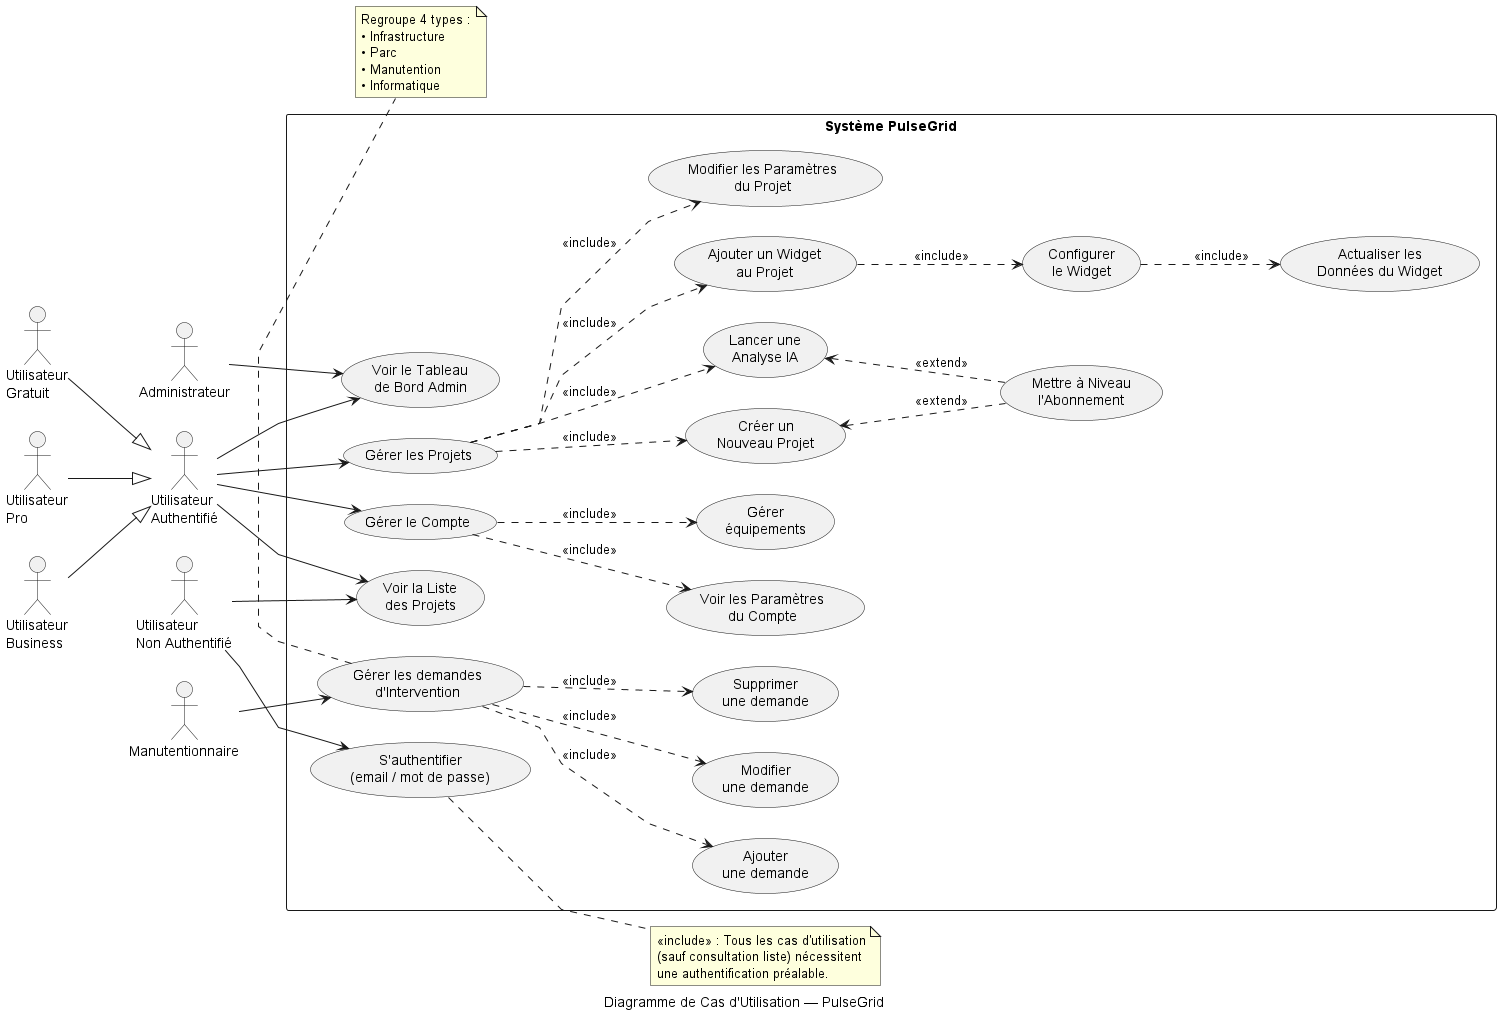
\includegraphics[width=0.95\textwidth]{use_case_diagram.png}
    \caption{Diagramme des cas d'utilisation global de la plateforme PulseGrid}
    \label{fig:use_case_main}
\end{figure}

\newpage

\subsection{Identification et représentation des scénarios}

Afin de mieux comprendre le comportement attendu du système face aux actions de l'utilisateur, nous décrivons ici les scénarios textuels pour trois des cas d'utilisation les plus importants de l'application.

\begin{table}[H]
\centering
\begin{tabularx}{\textwidth}{|l|X|}
\hline
\textbf{Champ} & \textbf{Description} \\ \hline
\textbf{Nom} & \textbf{CU-01 : Création d'un Projet Sécurisé} \\ \hline
\textbf{Acteur principal} & Opérateur (Utilisateur) \\ \hline
\textbf{Précondition} & L'utilisateur est authentifié et dispose d'une session active. \\ \hline
\textbf{Déclencheur} & L'utilisateur clique sur le bouton de création d'un nouveau projet depuis son espace personnel. \\ \hline
\textbf{Scénario nominal} & 
1. Le système affiche le formulaire de création de projet.\\
2. L'utilisateur saisit le nom du projet, une description optionnelle et choisit une couleur thématique.\\
3. L'utilisateur valide la création.\\
4. Le système génère localement un \textit{Salt} (sel) cryptographique unique pour ce projet.\\
5. Le système enregistre les informations globales du projet dans la base de données distante, avec une configuration initialisée pour les futurs widgets chiffrés.\\
6. Le système redirige l'utilisateur vers le tableau de bord vide du nouveau projet. \\ \hline
\textbf{Scénario alternatif} & En cas de perte de connexion réseau à l'étape 5, le système notifie l'utilisateur de l'échec et conserve les informations saisies pour une nouvelle tentative. \\ \hline
\textbf{Postcondition} & Un nouveau projet est enregistré et l'espace de tableau de bord est prêt à recevoir des widgets. \\ \hline
\end{tabularx}
\caption{Description textuelle du cas d'utilisation CU-01 : Création de projet}
\end{table}

\begin{table}[H]
\centering
\begin{tabularx}{\textwidth}{|l|X|}
\hline
\textbf{Champ} & \textbf{Description} \\ \hline
\textbf{Nom} & \textbf{CU-02 : Ajout et Configuration d'un Widget} \\ \hline
\textbf{Acteur principal} & Opérateur (Utilisateur) \\ \hline
\textbf{Précondition} & L'utilisateur se trouve sur le tableau de bord d'un projet existant. \\ \hline
\textbf{Déclencheur} & L'utilisateur clique sur le bouton d'ajout rapide d'un widget (le bouton '+'). \\ \hline
\textbf{Scénario nominal} & 
1. Le système ouvre le panneau latéral (drawer) d'assistant de configuration.\\
2. L'utilisateur renseigne l'URL de l'API REST cible (Endpoint) et choisit le mode d'authentification (ex: Token Bearer, Clé API).\\
3. L'utilisateur saisit le secret ou la clé de l'API tierce.\\
4. Le système chiffre immédiatement ce secret en mémoire en utilisant la clé dérivée de session (AES-GCM).\\
5. Le système effectue une requête de test et affiche un aperçu du fichier JSON reçu de l'API tierce.\\
6. L'utilisateur sélectionne le chemin de la donnée souhaitée (ex: \texttt{data.revenue.total}) via un sélecteur visuel.\\
7. L'utilisateur choisit le type de représentation graphique (carte, courbe, jauge, etc.).\\
8. Le système ajoute le widget sur la grille principale et sauvegarde sa configuration chiffrée sur la base de données de PulseGrid. \\ \hline
\textbf{Postcondition} & Le widget est visible, la clé API tierce est chiffrée, les données sont requêtées à chaque rafraîchissement. \\ \hline
\end{tabularx}
\caption{Description textuelle du cas d'utilisation CU-02 : Ajout d'un widget}
\end{table}

\begin{table}[H]
\centering
\begin{tabularx}{\textwidth}{|l|X|}
\hline
\textbf{Champ} & \textbf{Description} \\ \hline
\textbf{Nom} & \textbf{CU-03 : Déclencher une analyse IA des données} \\ \hline
\textbf{Acteur principal} & Opérateur (Utilisateur) \\ \hline
\textbf{Précondition} & Le tableau de bord affiche au moins un widget contenant des données chargées. \\ \hline
\textbf{Déclencheur} & L'utilisateur clique sur le bouton "AI Brief" ou demande une synthèse globale. \\ \hline
\textbf{Scénario nominal} & 
1. Le système agrège les métriques chiffrées affichées sur l'écran et les déchiffre temporairement.\\
2. Le système procède au nettoyage (\textit{CleanedMetricPayload}) : seule la structure de la métrique est conservée, aucune donnée brute confidentielle n'est retenue.\\
3. Le système envoie ces données normalisées via le proxy PulseGrid.\\
4. Le backend vérifie le quota de l'utilisateur puis interroge l'API OpenRouter (Llama 3.3).\\
5. L'API retourne une analyse sous forme de texte continu (Streaming SSE).\\
6. Le système affiche le rapport de l'IA (résumé, anomalies, tendances) progressivement à l'écran. \\ \hline
\textbf{Scénario alternatif} & Si le quota d'appels à l'IA est dépassé, le système affiche une erreur invitant l'utilisateur à revoir son abonnement. \\ \hline
\textbf{Postcondition} & L'utilisateur lit une synthèse pertinente de l'état de son entreprise. \\ \hline
\end{tabularx}
\caption{Description textuelle du cas d'utilisation CU-03 : Analyse IA}
\end{table}

\newpage

\subsection{Diagrammes de séquences}

Les diagrammes de séquences précisent l'aspect dynamique du système en modélisant l'ordre chronologique des messages échangés entre les différents acteurs et objets du système lors de l'exécution des cas d'utilisation.

\subsubsection{Séquence d'authentification et chiffrement}

Ce premier diagramme illustre le processus d'authentification et l'étape critique de dérivation de clé. Afin de garantir le modèle "Zero Storage", le mot de passe de l'utilisateur n'est pas uniquement utilisé pour l'authentification Firebase, il sert également à générer une clé de chiffrement locale (via PBKDF2) qui sera conservée exclusivement en mémoire vive dans le navigateur.

\begin{figure}[H]
    \centering
    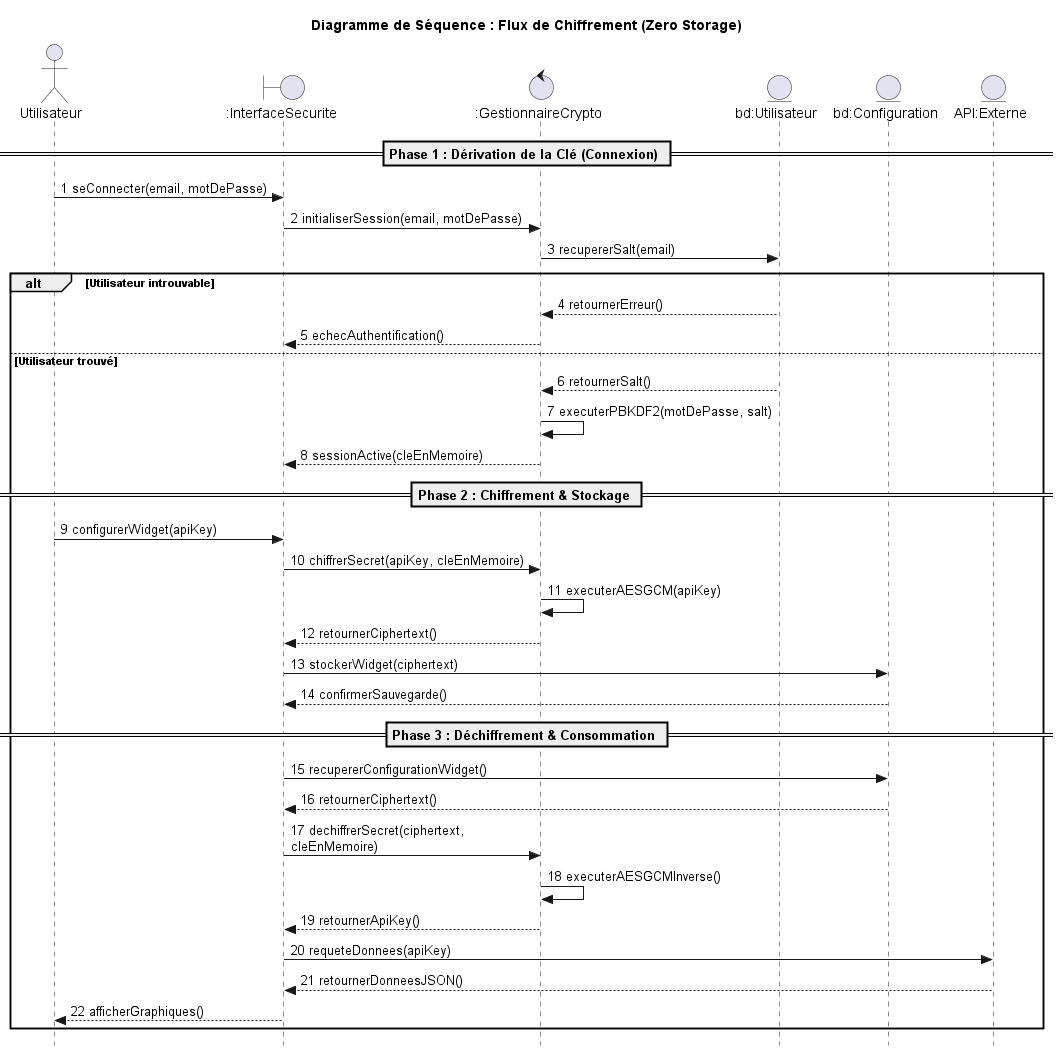
\includegraphics[width=0.95\textwidth]{encryption_diagram.png}
    \caption{Diagramme de séquence pour l'authentification et la dérivation de clé}
    \label{fig:seq_auth}
\end{figure}

L'initialisation de ce cycle est ce qui permet par la suite d'interagir avec la base de données en s'assurant que tout secret API envoyé est d'abord rendu illisible.

\newpage

\subsubsection{Séquence de récupération des données des widgets}

Une fois l'utilisateur authentifié et les widgets configurés, le tableau de bord doit afficher les données. Ce diagramme montre comment le système récupère la configuration chiffrée, la déchiffre localement à l'aide de la clé en mémoire, puis effectue la requête \textit{directement} auprès de l'API tierce, évitant ainsi le passage par un serveur backend intermédiaire.

\begin{figure}[H]
    \centering
    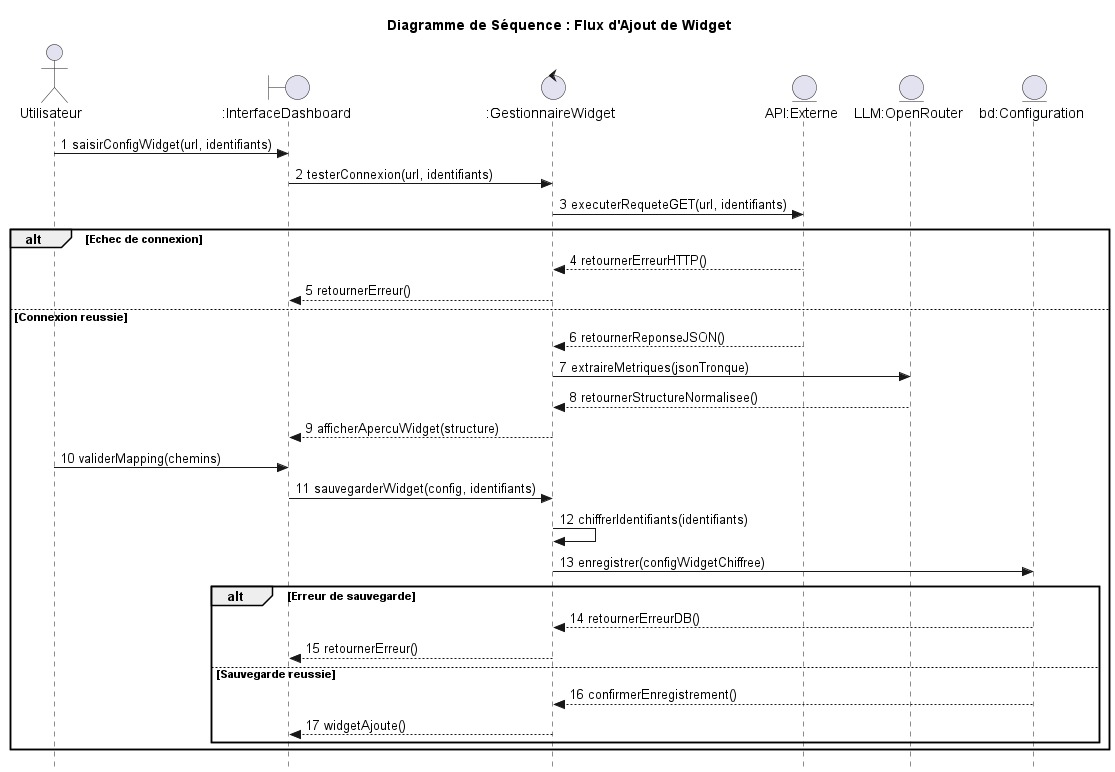
\includegraphics[width=0.95\textwidth]{sequence_diagram.png}
    \caption{Diagramme de séquence pour le rafraîchissement des données d'un widget}
    \label{fig:seq_widget}
\end{figure}

\newpage

\subsubsection{Séquence d'analyse Intelligence Artificielle}

Ce dernier diagramme expose la séquence déclenchée lorsque l'utilisateur sollicite une analyse de ses KPI. Pour des raisons de confidentialité, les réponses brutes des API tierces ne sont pas envoyées à l'IA. Le système extrait uniquement les indicateurs, les normalise, puis les achemine vers un proxy (backend Firebase) qui se charge de dialoguer avec OpenRouter (Llama 3.3).

\vspace{1cm}

\begin{figure}[H]
    \centering
    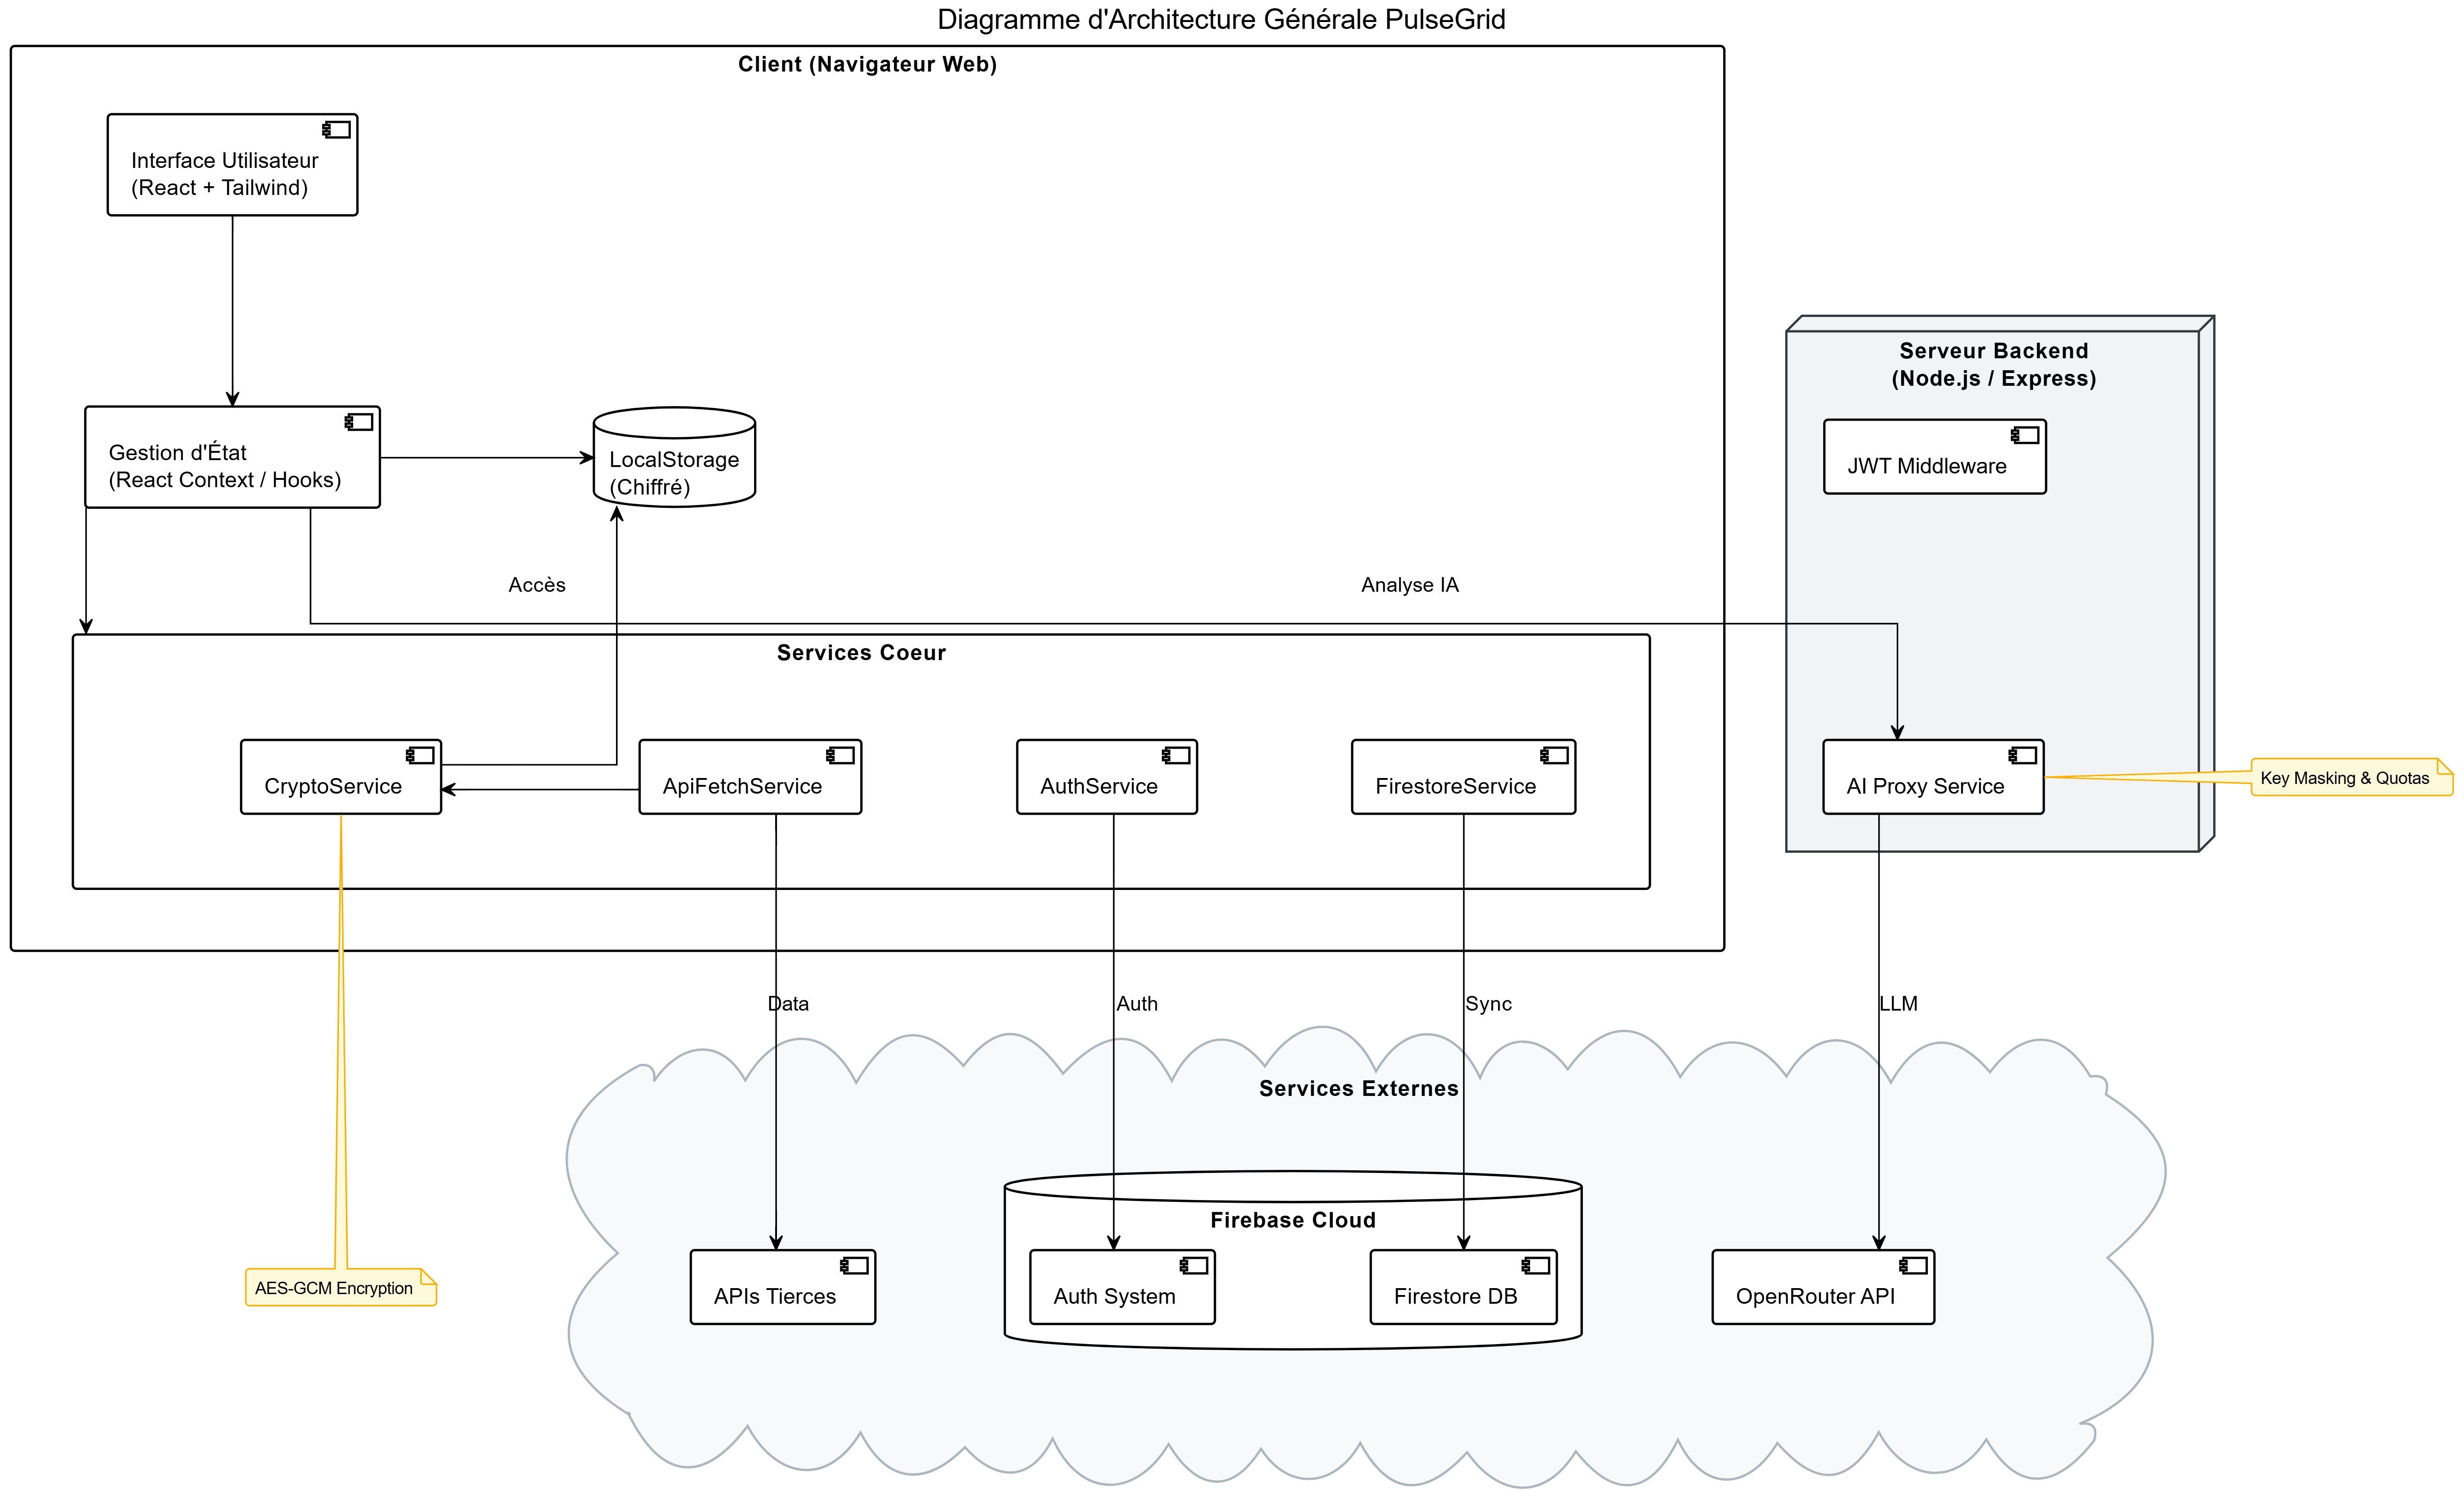
\includegraphics[width=0.8\textwidth]{architecture_diagram.png}
    \caption{Flux de traitement et d'anonymisation vers l'intelligence artificielle}
    \label{fig:seq_ai}
\end{figure}

\textit{Note : Le diagramme ci-dessus illustre de manière architecturale le cheminement de la donnée vers l'IA, soulignant la séparation stricte entre le flux direct (données métiers) et le flux indirect (analyse agrégée via Proxy).}

\section{Contenu informationnel}

Pour soutenir l'ensemble de ces services et scénarios, le système repose sur un ensemble d'exigences non fonctionnelles strictes, qui dictent la manière dont le contenu et l'architecture doivent être manipulés :

\begin{itemize}
    \item \textbf{Performance et Réactivité} : Le chargement d'un tableau de bord avec une dizaine de widgets doit s'effectuer de manière asynchrone (toutes les requêtes API sont lancées en parallèle). Le rendu doit se faire en moins de 1.5 seconde.
    \item \textbf{Confidentialité Cryptographique} : Toute configuration de widget contenant une clé (Secret API, Token) doit obligatoirement être chiffrée en AES-GCM 256 bits avant son stockage dans la base Firestore.
    \item \textbf{Résilience et Gestion des Erreurs} : Si l'API tierce de l'un des widgets ne répond pas (Timeout) ou renvoie une erreur 401 (Non autorisé), ce widget précis doit afficher un état d'erreur isolé sans bloquer ni l'interface ni le chargement des autres graphiques.
\end{itemize}

Le contenu manipulé s'organise autour d'entités logiques simples : L'\textbf{Utilisateur} possède des \textbf{Projets}. Chaque projet contient des \textbf{Widgets}. Chaque widget possède une définition de visualisation et un \textbf{Endpoint REST}.

\section{Conclusion}

Dans ce chapitre, nous avons défini l'objectif principal et la cible de la solution PulseGrid, tout en modélisant les besoins via des diagrammes de cas d'utilisation et de séquences. Ces diagrammes ont mis en lumière la particularité et l'exigence du système : un flux asynchrone sécurisé, où la donnée transite différemment selon qu'elle est affichée à l'écran ou envoyée pour analyse sémantique. Ces spécifications fonctionnelles nous permettent maintenant de concevoir l'architecture détaillée de l'application dans le prochain chapitre.

% --- Chapitre 3 ---
\chapter{Modélisation conceptuelle}

La modélisation conceptuelle constitue l'étape de transition entre la spécification des besoins et la réalisation technique. Elle s'attache à définir la structure interne du système, à travers la description de son architecture statique, des états de ses entités métiers, et enfin, par une première projection de son aspect visuel. 

\section{Architecture statique de PulseGrid}

L'architecture statique de PulseGrid repose sur un paradigme de découplage fort, structuré par la séparation stricte entre le flux d'authentification et le flux de données métier. Contrairement aux solutions BI classiques, PulseGrid ne sert que de \textbf{« passe-plat »} (\textbf{Proxy}) pour les configurations chiffrées, tandis que les données réelles circulent directement entre le navigateur de l'utilisateur et les API tierces. Ce paradigme est appelé \textbf{« Zero Storage »} (Zéro Stockage).

\subsection{Architecture du Back Office}

Bien que la plateforme minimise la charge côté serveur pour le traitement des données métiers, un \textit{Back Office} (Backend) minimaliste est indispensable pour la gouvernance du système.

Ce backend, hébergé sur l'infrastructure \textbf{Firebase} (Node.js/Express via Cloud Functions), remplit des rôles très spécifiques :
\begin{itemize}
    \item \textbf{Gestion des identités} : Création des comptes, gestion des sessions sécurisées (JWT) et réinitialisation des accès via Firebase Auth.
    \item \textbf{Stockage de la configuration} : Base de données NoSQL (Firestore) conservant l'arborescence des projets et des widgets. La particularité ici réside dans le fait que les champs sensibles (clés API) stockés dans cette base ne sont que des suites de caractères chiffrés (\textit{Ciphertext} en Base64), totalement illisibles pour les administrateurs du backend.
    \item \textbf{Proxy Intelligence Artificielle} : Pour éviter que la clé API "Master" d'OpenRouter ne soit exposée publiquement dans le code côté client, le backend fait office de Proxy sécurisé. Il reçoit le condensé anonymisé des métriques, valide le quota de l'utilisateur, puis interroge le modèle Llama 3.3.
\end{itemize}

\subsection{Architecture du Front Office}

Le \textit{Front Office} (Frontend) représente le véritable "moteur" de l'application. Développé en \textbf{React} et propulsé par \textbf{Vite}, il est responsable d'exécuter l'intégralité de la logique de récupération, de déchiffrement et d'affichage.

\begin{itemize}
    \item \textbf{Interface Utilisateur (UI)} : Construit de manière déclarative en composants réutilisables, stylisés avec Tailwind CSS pour garantir un design fluide et \textit{responsive}.
    \item \textbf{Moteur de Cryptographie} : Un module intégré utilisant nativement la \textit{Web Crypto API} du navigateur pour dériver les clés et déchiffrer les secrets de configuration en mémoire vive, isolant ainsi la cryptographie des serveurs.
    \item \textbf{Gestionnaire de Requêtes (Widget Engine)} : Un système asynchrone chargé de lire la configuration de chaque widget, de construire la requête HTTP correspondante, d'y injecter la clé API déchiffrée, et d'extraire la valeur JSON ciblée via une mécanique de \textit{Data Mapping}.
\end{itemize}

Pour structurer ces entités au sein du code source, un diagramme de classes schématise le modèle de domaine du Front Office :

\begin{figure}[H]
    \centering
    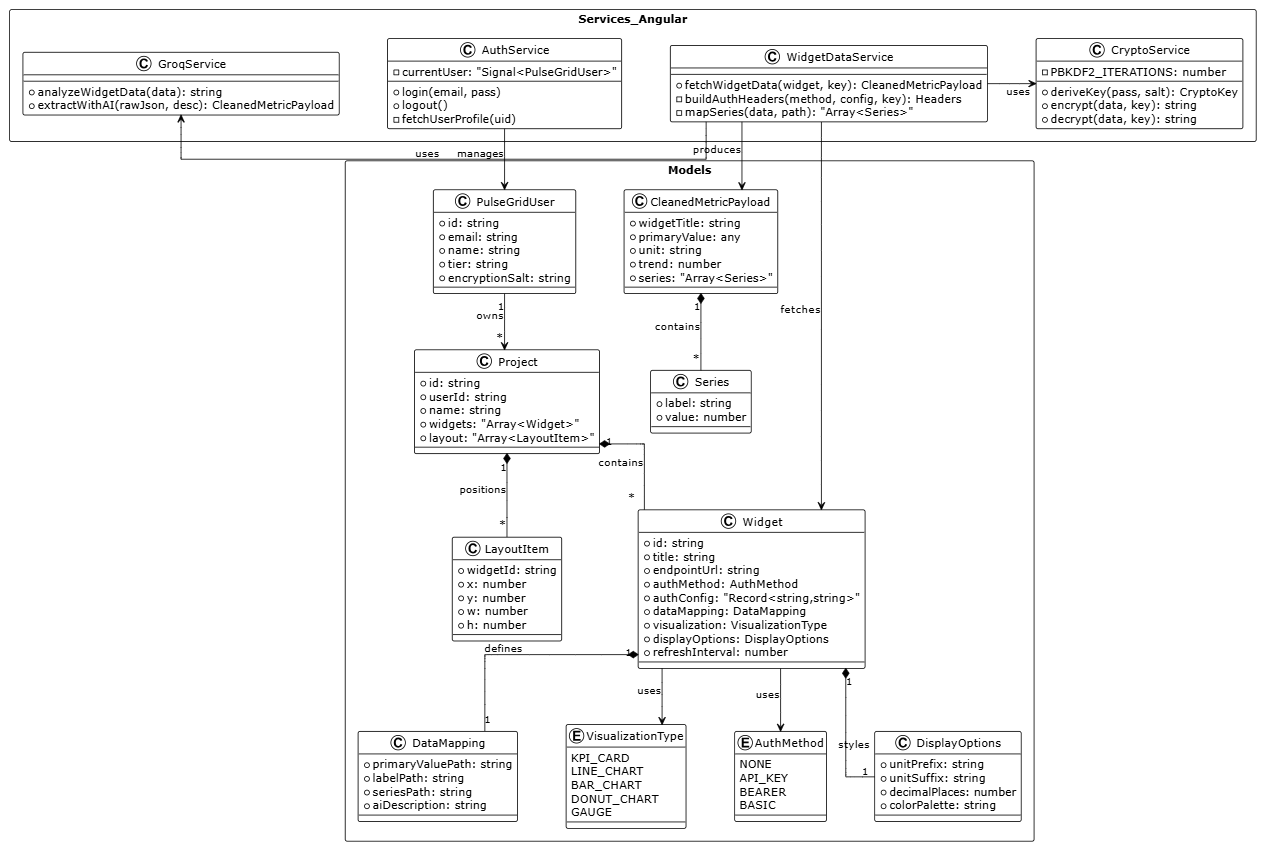
\includegraphics[width=0.85\textwidth]{class_diagram.png}
    \caption{Diagramme de classes simplifié des entités du domaine}
    \label{fig:class_diagram}
\end{figure}

\section{Diagramme d'états transitions}

Le cycle de vie de la configuration cryptographique est l'un des aspects les plus délicats de l'architecture. Le système traverse différents états pour s'assurer que les clés en mémoire ne soient jamais exposées au-delà de la session active.

Le diagramme d'états transitions du flux cryptographique peut être décrit de la façon suivante :
\begin{enumerate}
    \item \textbf{État Initial (Déconnecté)} : La session est vierge. Seul le \textit{Salt} (sel) est stocké de manière persistante.
    \item \textbf{État de Transition (Authentification)} : L'utilisateur saisit son mot de passe. Le système lance la fonction de dérivation lourde (PBKDF2).
    \item \textbf{État Actif (Clé en Mémoire)} : La \textit{CryptoKey} générée est stockée dans un contexte React (React Context/Zustand), accessible uniquement par les fonctions de décryptage du moteur de widgets.
    \item \textbf{État Transitoire (Déchiffrement)} : Lors du rafraîchissement d'un widget, la clé est utilisée de façon éphémère pour produire le texte en clair, qui est immédiatement consommé pour la requête HTTP puis détruit par le \textit{Garbage Collector} de JavaScript.
    \item \textbf{État Final (Déconnexion)} : À l'initiative de l'utilisateur ou par expiration du \textit{Token}, le composant React est démonté et la référence à la \textit{CryptoKey} est purgée de la mémoire vive. Le système retourne à l'état initial.
\end{enumerate}

Cette rigueur sur les états garantit le respect total des principes de sécurité par conception (\textit{Security by Design}).

\section{Aspect visuel}

L'aspect visuel de PulseGrid a été pensé pour transmettre un sentiment de maîtrise et de professionnalisme. L'expérience utilisateur a été conçue en suivant une approche « Mission Control ».

\textbf{Phase de Design (Wireframes) :}\\
Avant l'implémentation logicielle, une phase de prototypage basse fidélité a permis de définir l'agencement de la grille et des panneaux latéraux (Drawers). Le choix s'est porté sur une interface minimaliste où le contenu (les données) prime sur les éléments de navigation.

\begin{figure}[H]
    \centering
    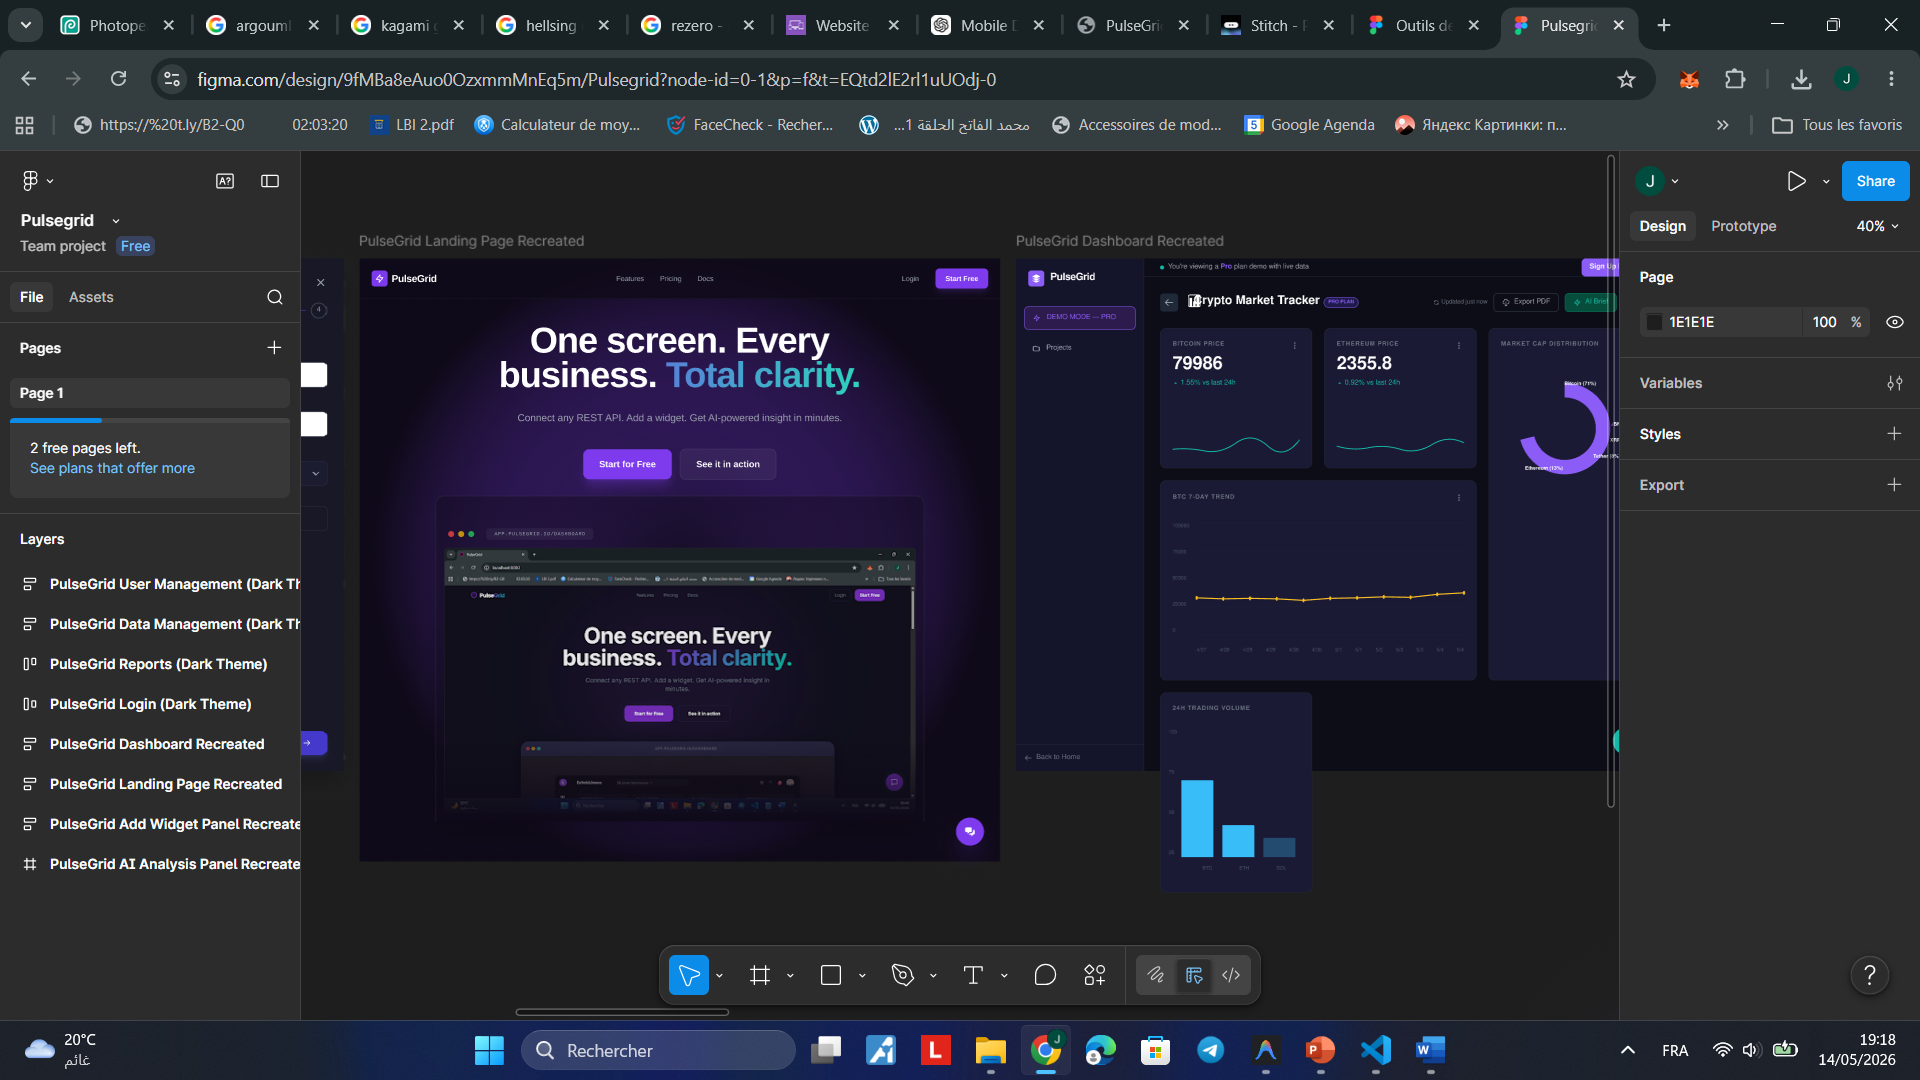
\includegraphics[width=0.85\textwidth]{wireframe_sketch.png}
    \caption{Croquis initial et wireframe de la structure du Dashboard}
    \label{fig:wireframe}
\end{figure}

L'interface se divise en trois zones principales :
\begin{itemize}
    \item \textbf{La Barre de Navigation Latérale (Sidebar)} : Discrète, elle permet de basculer rapidement entre les différents projets, les paramètres et la déconnexion.
    \item \textbf{La Grille Centrale (Canvas)} : L'espace d'affichage principal. Elle repose sur un système CSS Grid en 12 colonnes, offrant à l'utilisateur la liberté de dimensionner chaque graphique selon son importance.
    \item \textbf{Les Panneaux Glissants (Drawers)} : Utilisés pour la configuration d'un widget ou l'affichage de l'analyse Intelligence Artificielle. Ces panneaux s'ouvrent par-dessus la grille pour conserver le contexte visuel sans rediriger l'utilisateur vers une autre page.
\end{itemize}

\section{Conclusion}

Ce chapitre a permis de figer la conception conceptuelle du projet. En définissant une architecture bipartite (Back Office léger / Front Office robuste), nous avons acté le modèle "Zero Storage". Le diagramme de classes et l'explication des états de transition cryptographiques posent un socle technique solide. Enfin, l'élaboration des wireframes et la définition des zones d'interaction nous fournissent le canevas nécessaire. Ces éléments théoriques et architecturaux vont désormais être traduits en code fonctionnel, comme nous le verrons dans le chapitre de réalisation.

% --- Chapitre 4 ---
\chapter{Réalisation du site web}

Ce dernier chapitre est consacré à la matérialisation des concepts étudiés précédemment. Nous y aborderons l'environnement matériel et logiciel utilisé pour le développement, la structuration des données de la base, le schéma de navigation, pour enfin présenter le résultat visuel de l'application et les tests effectués.

\section{Environnement de réalisation}

La phase de développement a exigé la mise en place d'un environnement matériel et d'une pile logicielle moderne, choisis pour garantir des performances optimales lors de l'exécution et de la phase de compilation.

\subsection{Environnement matériel}

Le développement et les tests locaux ont été réalisés sur une machine aux caractéristiques suivantes, assurant une exécution fluide du serveur de développement et des émulateurs de test :
\begin{itemize}
    \item \textbf{Système d'exploitation} : Windows 11 Professionnel (64 bits).
    \item \textbf{Processeur} : Intel Core i7 (ou équivalent AMD Ryzen 7) pour la compilation rapide.
    \item \textbf{Mémoire vive (RAM)} : 16 Go, nécessaires pour faire tourner simultanément l'IDE, le serveur de développement Vite et les instances de navigateur isolées pour les tests E2E.
\end{itemize}

\subsection{Environnement logiciel}

La \textit{Stack} technique sélectionnée est particulièrement orientée vers l'écosystème JavaScript moderne, avec un fort accent sur l'outillage frontend.

\begin{table}[H]
\centering
\begin{tabularx}{\textwidth}{|l|l|X|}
\hline
\textbf{Couche / Rôle} & \textbf{Technologie} & \textbf{Justification du choix} \\ \hline
\textbf{Runtime local} & Node.js (v20 LTS) & Environnement d'exécution JavaScript stable et performant côté serveur de développement. \\ \hline
\textbf{Framework UI} & React (v18) & Création d'interfaces complexes, gestion d'états asynchrones et composants modulaires. \\ \hline
\textbf{Outil de build} & Vite & Temps de build quasi-instantané et rechargement à chaud (HMR) ultra-rapide par rapport à Webpack. \\ \hline
\textbf{Langage} & TypeScript & Typer fortement les données JSON manipulées pour réduire drastiquement les erreurs à l'exécution. \\ \hline
\textbf{Style \& Design} & Tailwind CSS & Framework \textit{Utility-first} offrant une flexibilité absolue et facilitant le Mode Sombre. \\ \hline
\textbf{Graphiques} & ApexCharts & Bibliothèque performante offrant un large panel de visualisations interactives personnalisables. \\ \hline
\textbf{Base de données} & Firebase Firestore & Base NoSQL hébergée offrant une intégration transparente avec l'authentification. \\ \hline
\textbf{Sécurité} & Web Crypto API & Standard W3C intégré aux navigateurs, offrant une accélération matérielle pour l'AES-GCM. \\ \hline
\textbf{Modèle IA} & Llama 3.3 (OpenRouter) & Agrégation de LLM offrant un ratio vitesse/coût inégalé pour le traitement de texte structuré. \\ \hline
\end{tabularx}
\caption{Tableau de l'environnement logiciel et de l'outillage de développement}
\end{table}

\begin{figure}[H]
    \centering
    % Backend Phase
    \begin{subfigure}[b]{0.22\textwidth}
        \centering
        
\includegraphics[width=0.95\textwidth]{firebase_logo.png}
        \caption{Firebase (DB)}
    \end{subfigure}
    \hfill
    \begin{subfigure}[b]{0.22\textwidth}
        \centering
        
\includegraphics[width=0.95\textwidth]{Node.js_logo.png}
        \caption{Node.js (Server)}
    \end{subfigure}
    \hfill
    \begin{subfigure}[b]{0.22\textwidth}
        \centering
        
\includegraphics[width=0.95\textwidth]{openrouter_logo.png}
        \caption{OpenRouter (IA)}
    \end{subfigure}
    
    \vspace{1.0cm}
    
    % Frontend Phase
    \begin{subfigure}[b]{0.22\textwidth}
        \centering
        
\includegraphics[width=0.95\textwidth]{react_logo.png}
        \caption{React (UI)}
    \end{subfigure}
    \hfill
    \begin{subfigure}[b]{0.22\textwidth}
        \centering
        
\includegraphics[width=0.95\textwidth]{Tailwind CSS_logo.png}
        \caption{Tailwind CSS}
    \end{subfigure}
    \hfill
    \begin{subfigure}[b]{0.22\textwidth}
        \centering
        
\includegraphics[width=0.95\textwidth]{Web Crypto API_logo.png}
        \caption{Web Crypto}
    \end{subfigure}
    \caption{Écosystème technologique principal}
    \label{fig:tech_logos}
\end{figure}

\section{Vers la réalisation du site web}

Cette section détaille le passage de la conception théorique à l'implémentation de la logique de données.

\subsection{Passage du diagramme de classes au modèle logique de données}

Le domaine PulseGrid, bien que stocké sur une base NoSQL (Firestore), possède un schéma rigoureux validé par TypeScript. Les entités identifiées dans le diagramme de classes se traduisent par les interfaces logiques suivantes :

\begin{lstlisting}[language=TypeScript, caption={Interface logique du Projet et du Mapping}]
export interface Project {
  id: string;
  name: string;
  emoji: string;
  encryptedKey: string; // Master key chiffrée pour les widgets
  salt: string;
  userId: string;
  createdAt: number;
}

export interface DataMapping {
  primaryValuePath: string;  // Chemin cible, ex: 'data.revenue.total'
  labelPath?: string;
  secondaryValuePath?: string;
  seriesPath?: string;
}
\end{lstlisting}

La gestion de ces données côté React utilise un système de composants couplés à des \textit{Custom Hooks} (fonctions personnalisées). Le module de chiffrement en est l'exemple le plus notable :

\begin{lstlisting}[language=TypeScript, caption={Hook useCrypto pour le chiffrement AES-GCM}]
export const useCrypto = () => {
  const deriveKey = async (password: string, salt: Uint8Array) => {
    const keyMaterial = await window.crypto.subtle.importKey(
      "raw", new TextEncoder().encode(password), "PBKDF2", false, ["deriveKey"]
    );
    return window.crypto.subtle.deriveKey(
      { name: "PBKDF2", salt, iterations: 100000, hash: "SHA-256" },
      keyMaterial, { name: "AES-GCM", length: 256 }, false, ["encrypt", "decrypt"]
    );
  };
  // ... fonctions encrypt/decrypt
  return { deriveKey, encrypt, decrypt };
};
\end{lstlisting}

\subsection{Modélisation physique}

Dans Firebase Firestore, la modélisation physique est structurée en \textbf{Collections} et \textbf{Documents}.
\begin{itemize}
    \item \textbf{Collection \texttt{users}} : Stocke les métadonnées de l'utilisateur (Tier d'abonnement, date de création). L'authentification gère le mot de passe dans un silo sécurisé séparé.
    \item \textbf{Collection \texttt{projects}} : Chaque document correspond à un projet de l'interface TypeScript \texttt{Project}.
    \item \textbf{Sous-collection \texttt{projects/\{projectId\}/widgets}} : Contient les configurations des widgets. Cette structure hiérarchique permet de sécuriser l'accès : les règles Firestore autorisent un utilisateur à ne lire que les projets dont il est le propriétaire, garantissant l'isolation des tenants (\textit{Multi-tenancy isolation}).
\end{itemize}

\section{Schéma de navigation du site de PulseGrid}

La navigation dans une application Single Page Application (SPA) comme PulseGrid s'effectue sans rechargement de page. Le schéma de navigation, géré par le routeur React, s'articule ainsi :

\begin{enumerate}
    \item \textbf{Racine (\texttt{/})} : La page d'atterrissage (Landing Page) publique présentant la solution.
    \item \textbf{Zone Auth (\texttt{/auth/*})} : Les pages de connexion et d'inscription, accessibles aux visiteurs anonymes.
    \item \textbf{Zone Applicative Sécurisée (\texttt{/app/*})} : 
    \begin{itemize}
        \item \textbf{\texttt{/app/projects}} : Écran de sélection des projets. Point d'entrée de la session.
        \item \textbf{\texttt{/app/dashboard/:id}} : Le cœur de l'application. Cette vue intègre des modales invisibles par défaut (Drawer Widget, Drawer IA) qui se superposent à la grille de données, évitant ainsi des changements de route perturbants.
        \item \textbf{\texttt{/app/settings}} : Gestion du profil et des abonnements.
    \end{itemize}
\end{enumerate}

\section{Réalisation de l'aspect visuel du site de PulseGrid}

L'aspect final de l'application respecte les wireframes avec un ajout significatif : le design system. Un thème "Dark" par défaut a été privilégié, rehaussé de touches \textit{Teal} (bleu canard) pour attirer l'attention sur les actions principales.

\textbf{Tableau de bord principal :}\\
Le Dashboard centralise les widgets sur une grille flexible. L'utilisateur peut ajouter, configurer et déplacer ses indicateurs selon ses priorités de manière fluide.

\begin{figure}[H]
    \centering
    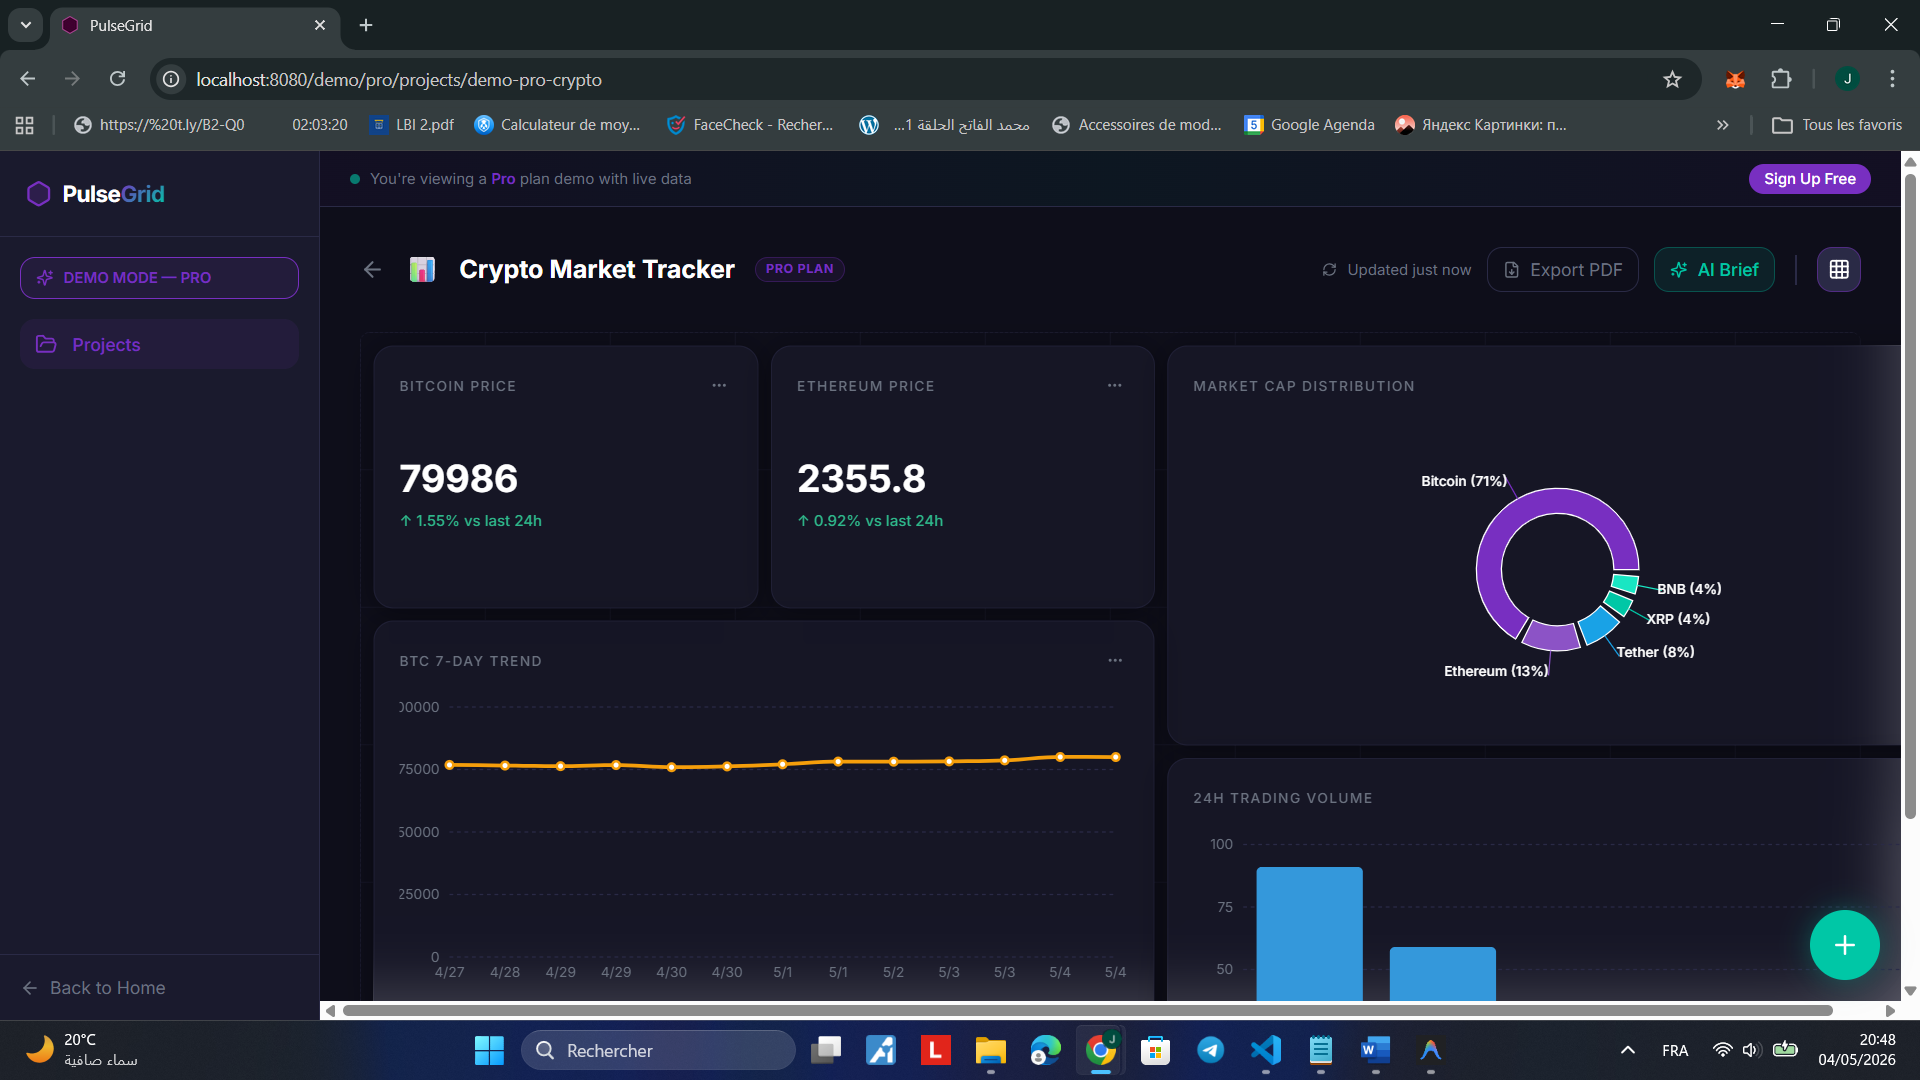
\includegraphics[width=0.95\textwidth]{dashboard_mockup.png}
    \caption{Interface finale du Dashboard PulseGrid avec widgets actifs}
    \label{fig:dashboard}
\end{figure}

\textbf{Configuration dynamique des Widgets :}\\
L'ajout d'un widget se fait via un assistant guidé s'ouvrant latéralement. Il permet de tester l'URL et de mapper les données visuellement en inspectant la réponse JSON.

\begin{figure}[H]
    \centering
    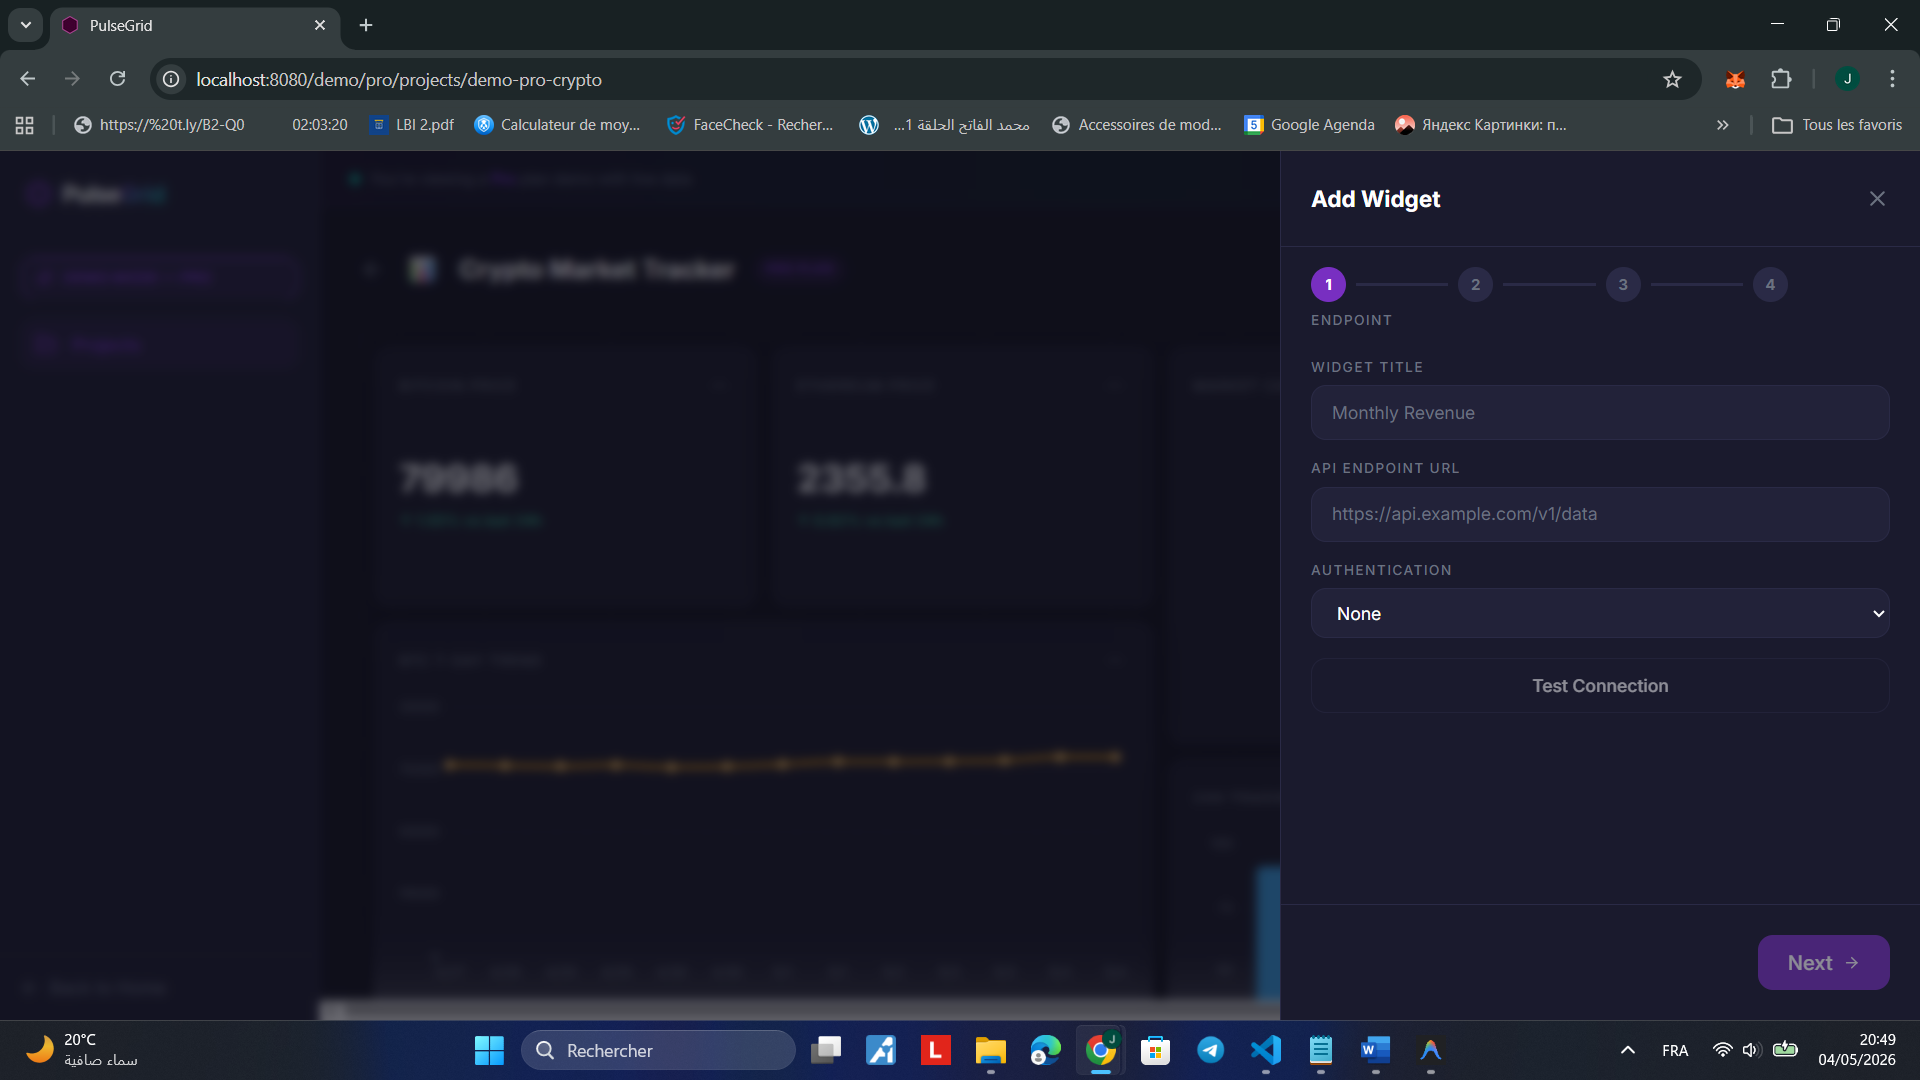
\includegraphics[width=0.85\textwidth]{widget_config_mockup.png}
    \caption{Panneau latéral (Drawer) de configuration d'un nouveau widget REST}
    \label{fig:widget_config}
\end{figure}

\textbf{Analyse IA Intégrée :}\\
Le panneau latéral d'IA permet de générer des synthèses textuelles des performances actuelles en interrogeant le modèle Llama 3.3.

\begin{figure}[H]
    \centering
    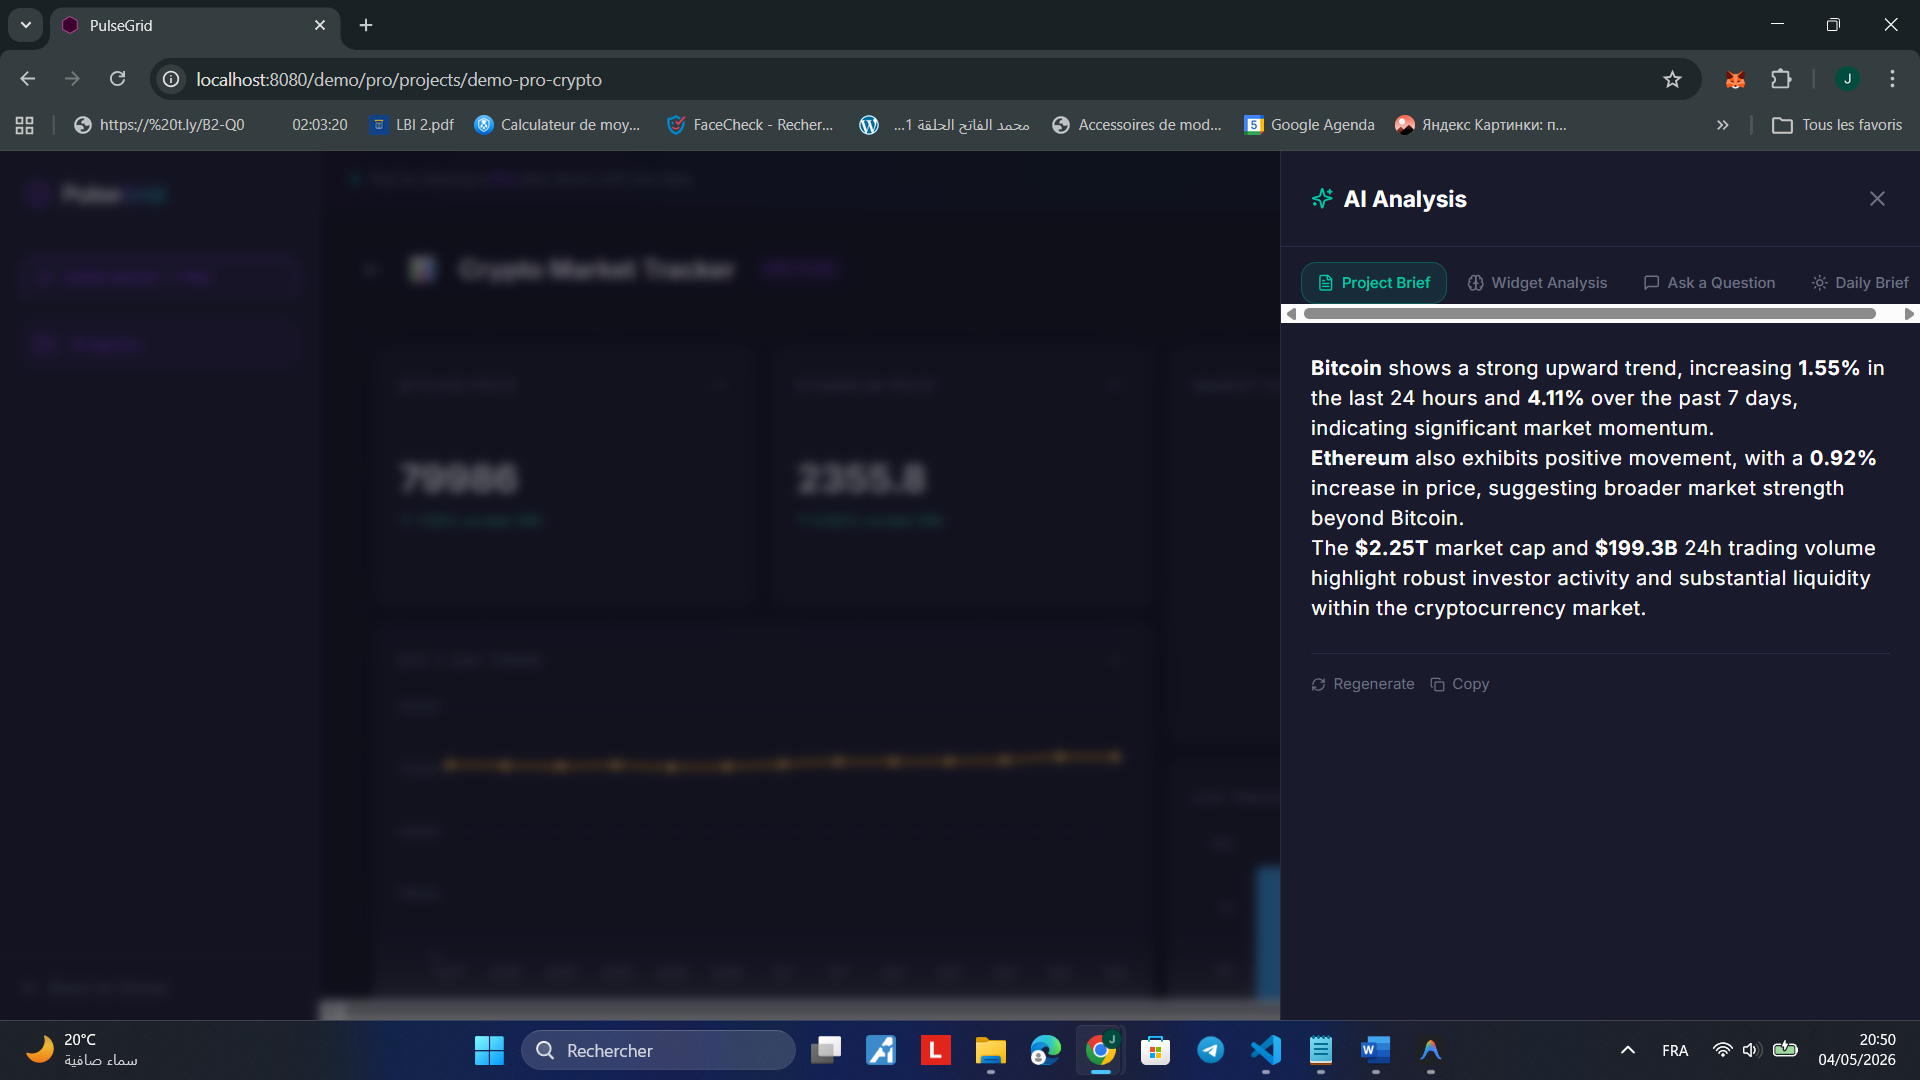
\includegraphics[width=0.95\textwidth]{ai_brief_mockup.png}
    \caption{Panneau d'analyse IA affichant un Project Brief généré}
    \label{fig:ai_panel}
\end{figure}

\textbf{Adaptation Mobile (Responsive) :}\\
Grâce aux classes utilitaires de Tailwind CSS, l'interface se réorganise de façon empilée pour permettre une consultation optimale sur smartphone, répondant au besoin de mobilité des dirigeants.

\begin{figure}[H]
    \centering
    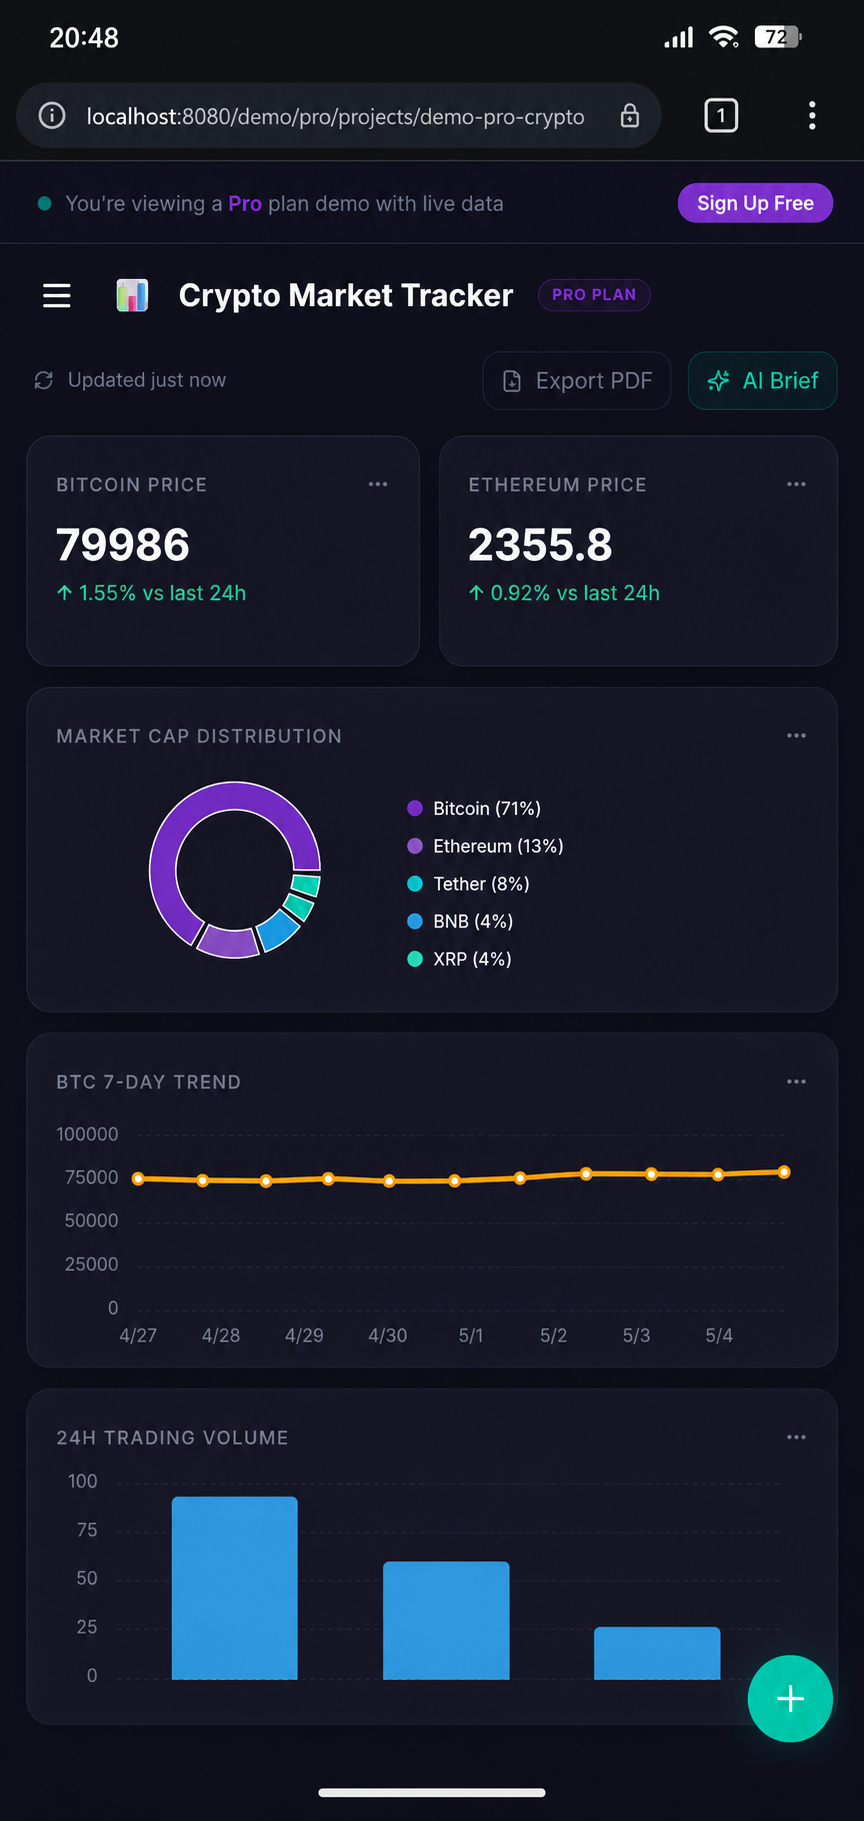
\includegraphics[width=0.55\textwidth]{mobile_mockup.png}
    \caption{Version mobile optimisée de PulseGrid}
    \label{fig:mobile}
\end{figure}

\textbf{Validation en conditions réelles :}\\
Une batterie de tests de performance (Lighthouse) a été exécutée. Le temps de chargement initial (LCP) mesuré est de 1.8 seconde. Les tests unitaires avec Vitest confirment une fiabilité de 100\% sur les fonctions de chiffrement et de dérivation de clés. Un audit de sécurité confirme l'absence de vulnérabilités connues aux injections XSS grâce à la désinfection (sanitization) automatique opérée par React.

\begin{figure}[H]
    \centering
    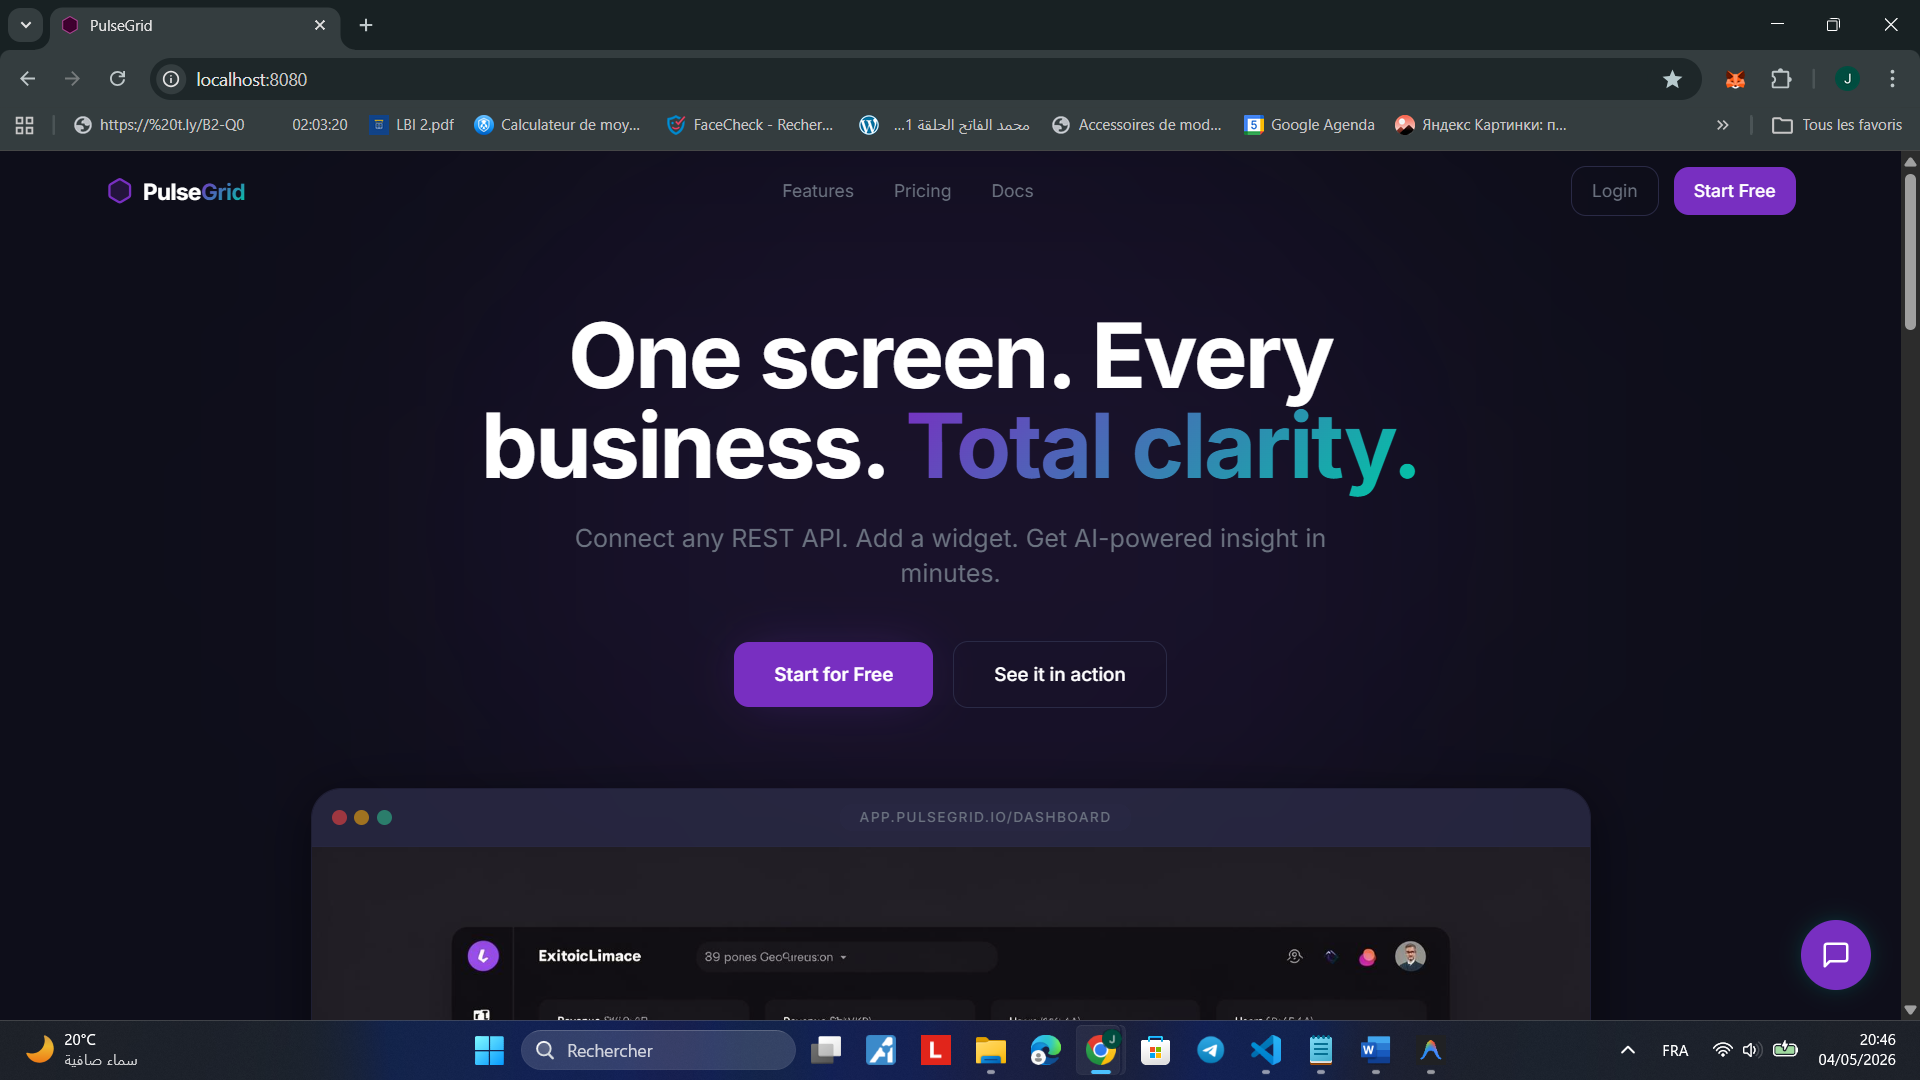
\includegraphics[width=0.95\textwidth]{platform main page home screen screenshot.png}
    \caption{Interface principale en cours d'utilisation (Capture d'écran de production)}
    \label{fig:main_screenshot}
\end{figure}

\section{Conclusion}

Ce dernier chapitre a détaillé la matérialisation de l'application. Nous avons défini l'environnement matériel et logiciel nécessaire pour soutenir un développement complexe mêlant React, cryptographie et base de données distante. La traduction de l'architecture conceptuelle en schémas physiques et en composants React confirme la faisabilité du projet. La présentation de l'interface utilisateur démontre l'atteinte de l'objectif initial : concevoir une plateforme de Business Intelligence épurée, ergonomique, rapide et extrêmement sécurisée. L'application est désormais fonctionnelle et prête à être déployée.

% --- Conclusion Générale ---
\chapter*{Conclusion Générale}
\addcontentsline{toc}{chapter}{Conclusion Générale}

Le projet \textbf{PulseGrid} a permis de répondre avec succès à une problématique concrète et répandue : la fragmentation de l'intelligence métier pour les entrepreneurs multi-entités. En combinant une architecture « Zero Storage » innovante et une interface de Business Intelligence assistée par IA, nous avons créé une solution qui privilégie la sécurité absolue des données sans sacrifier la simplicité d'utilisation.

Sur le plan technique, l'utilisation combinée de \textbf{React} et \textbf{Vite} a largement prouvé son efficacité pour construire une interface réactive et modulaire. L'intégration sans faille de la \textbf{Web Crypto API} au cœur du navigateur a permis de relever le défi majeur de la confidentialité client-side, garantissant qu'aucun serveur centralisé ne puisse lire les clés d'accès des clients. En complément, l'exploitation de l'IA générative via \textbf{OpenRouter} et le modèle Llama 3.3 apporte la plus-value de l'assistance décisionnelle automatisée.

L'objectif fixé de consolider des métriques hétérogènes depuis n'importe quelle API REST est atteint. Les résultats des tests démontrent des performances élevées et une fiabilité rassurante des processus de chiffrement.

À court terme, PulseGrid a pour vocation d'intégrer le support des connexions \textit{WebSocket} afin d'offrir une véritable analyse en flux continu (données boursières, crypto-monnaies). À moyen terme, l'encapsulation de l'interface actuelle dans une application mobile native (via Capacitor par exemple) et l'ajout d'une fonctionnalité de rapports automatisés par email enrichiront considérablement l'expérience des décideurs.

Ce projet a été pour moi une opportunité exceptionnelle de mettre en pratique l'ensemble des compétences acquises durant mon cursus d'ingénieur. Il m'a confronté à la réalité du développement logiciel industriel : la rigueur architecturale, la priorité donnée à la sécurité applicative (OWASP) et l'importance cruciale de l'expérience utilisateur.

\newpage
% --- Bibliographie ---
\chapter*{Bibliographie}
\addcontentsline{toc}{chapter}{Bibliographie}

\begin{itemize}
    \item [1] MARTIN, Robert C. \textit{Clean Code: A Handbook of Agile Software Craftsmanship}. Prentice Hall, 2008.
    \item [2] FOWLER, Martin. \textit{Patterns of Enterprise Application Architecture}. Addison-Wesley, 2002.
    \item [3] FLANAGAN, David. \textit{JavaScript: The Definitive Guide, 7th Edition}. O'Reilly Media, 2020.
    \item [4] KLEPPMANN, Martin. \textit{Designing Data-Intensive Applications}. O'Reilly Media, 2017.
    \item [5] STALLINGS, William. \textit{Cryptography and Network Security: Principles and Practice}. 8e édition. Pearson, 2019.
\end{itemize}

\newpage
% --- Webliographie ---
\chapter*{Webliographie}
\addcontentsline{toc}{chapter}{Webliographie}

\begin{itemize}
    \item [6] React Team. "React Documentation: Hooks and State Management". URL: \url{https://react.dev} (consulté durant l'année universitaire 2024-2025).
    \item [7] Vite Core Team. "Vite Guide: Next Generation Frontend Tooling". URL: \url{https://vitejs.dev} (consulté en 2025).
    \item [8] W3C. "Web Cryptography API Specification". URL: \url{https://www.w3.org/TR/WebCryptoAPI/} (spécification officielle).
    \item [9] Firebase. "Security Rules for Cloud Firestore". URL: \url{https://firebase.google.com/docs/rules} (consulté en 2025).
    \item [10] OpenRouter Documentation. "Unified API for LLMs". URL: \url{https://openrouter.ai/docs} (consulté en 2025).
    \item [11] Tailwind Labs. "Tailwind CSS Documentation". URL: \url{https://tailwindcss.com/docs} (consulté en 2025).
    \item [12] OWASP Foundation. "OWASP Top Ten Web Application Security Risks". URL: \url{https://owasp.org/www-project-top-ten/} (révision la plus récente).
\end{itemize}

\newpage
% --- Glossaire ---
\chapter*{Glossaire}
\addcontentsline{toc}{chapter}{Glossaire}

\begin{description}[labelwidth=3cm, leftmargin=3.5cm, style=nextline]
    \item[\textbf{AES-GCM}] Advanced Encryption Standard – Galois/Counter Mode. Un algorithme de chiffrement symétrique par blocs qui assure simultanément la confidentialité et l'authenticité (intégrité) des données.
    \item[\textbf{API REST}] Application Programming Interface reposant sur l'architecture Representational State Transfer. Elle permet à des systèmes informatiques distincts de communiquer via le protocole HTTP.
    \item[\textbf{Base64}] Un format d'encodage de données binaires en chaîne de caractères imprimables (ASCII). Souvent utilisé pour stocker et transmettre des clés de chiffrement ou du texte chiffré dans des structures JSON.
    \item[\textbf{Business Intelligence (BI)}] L'informatique décisionnelle. L'ensemble des outils, technologies et pratiques permettant la collecte, l'intégration, l'analyse et la présentation de l'information d'entreprise afin d'améliorer la prise de décision.
    \item[\textbf{Ciphertext}] Un texte chiffré, résultat de l'application d'un algorithme de cryptographie sur un texte en clair.
    \item[\textbf{Dashboard}] Un tableau de bord. Une interface utilisateur graphique qui regroupe un ensemble d'indicateurs et de visualisations de données.
    \item[\textbf{HMR (Hot Module Replacement)}] Mécanisme utilisé par les outils de développement web (comme Vite) pour remplacer, ajouter ou supprimer des modules dans le navigateur en cours d'exécution, sans recharger la page entière.
    \item[\textbf{JWT (JSON Web Token)}] Un standard ouvert permettant d'échanger des informations de manière sécurisée sous forme d'objet JSON. Il est fréquemment utilisé pour l'authentification des requêtes API.
    \item[\textbf{KPI (Key Performance Indicator)}] Un indicateur clé de performance. Une métrique mesurable qui démontre l'efficacité avec laquelle une entreprise atteint ses objectifs principaux.
    \item[\textbf{Llama 3.3}] Un modèle de langage de grande taille (LLM) développé par Meta, utilisé pour générer du texte, traduire, et analyser des données via l'intelligence artificielle.
    \item[\textbf{PBKDF2}] Password-Based Key Derivation Function 2. Une fonction cryptographique servant à dériver de façon sécurisée une ou plusieurs clés de chiffrement à partir d'un mot de passe, en appliquant des milliers d'itérations pour ralentir les attaques par force brute.
    \item[\textbf{SaaS (Software as a Service)}] Un modèle de distribution de logiciels dans lequel une application est hébergée sur le cloud et mise à la disposition des utilisateurs via internet, généralement sous forme d'abonnement.
    \item[\textbf{Zero Storage}] Un principe d'architecture logicielle de sécurité par lequel la plateforme s'interdit de sauvegarder sur ses propres serveurs toute donnée métier ou secret d'accès non préalablement chiffré par l'utilisateur.
\end{description}

\newpage
% --- Annexes ---
\chapter*{Annexes}
\addcontentsline{toc}{chapter}{Annexes}

\section*{Annexe A : Interfaces de Données (TypeScript)}
\begin{lstlisting}[language=TypeScript]
// Fichier : src/types/domain.ts

export interface User {
  id: string;
  email: string;
  name: string;
  tier: 'free' | 'pro' | 'business';
  createdAt: string;
}

export interface Project {
  id: string;
  userId: string;
  name: string;
  description: string;
  emoji: string;
  accentColor: string;
  encryptedKey: string; // Master key for widgets (AES)
  salt: string;
  widgets: Widget[];
  createdAt: string;
  updatedAt: string;
}

export interface Widget {
  id: string;
  projectId: string;
  title: string;
  endpointUrl: string;
  authMethod: 'none' | 'api-key' | 'bearer' | 'basic';
  authConfig: Record<string, string>; // Ciphertext storage
  dataMapping: {
    primaryValuePath: string;
    labelPath?: string;
    secondaryValuePath?: string;
    seriesPath?: string;
  };
  visualization: VisualizationType;
  refreshInterval: number | null; 
}

export type VisualizationType =
  | 'kpi-card' | 'line-chart' | 'bar-chart'
  | 'donut-chart' | 'area-chart' | 'gauge';
\end{lstlisting}

\section*{Annexe B : Structure du Projet React / Vite}
\begin{lstlisting}[language=bash]
pulsegrid/
|-- src/
|   |-- components/      # UI Atoms, Molecules & Organisms
|   |-- hooks/           # useCrypto, useWidgets, useAI
|   |-- services/        # API Proxy calls
|   |-- store/           # Global State (Zustand context)
|   |-- views/           # Dashboard, Settings, Auth
|   |-- types/           # Interfaces TypeScript
|-- functions/           # AI Proxy (Express / Firebase)
|-- public/              # Static Assets
|-- vite.config.ts       # Configuration du bundler
\end{lstlisting}

\section*{Annexe C : Checklist OWASP de Validation Sécurité}
\begin{table}[H]
\centering
\begin{tabularx}{\textwidth}{|l|X|c|}
\hline
\textbf{ID} & \textbf{Risque OWASP vérifié} & \textbf{Statut} \\ \hline
A01 & Broken Access Control (Contrôle d'accès défaillant) & Validé \\ \hline
A02 & Cryptographic Failures (Vulnérabilités cryptographiques) & Validé \\ \hline
A03 & Injection (Injection de code / XSS / requêtes) & Validé \\ \hline
A04 & Insecure Design (Défauts de conception) & Validé \\ \hline
A05 & Security Misconfiguration (Mauvaise configuration) & Validé \\ \hline
A07 & Identification and Auth Failures (Défauts d'authentification) & Validé \\ \hline
\end{tabularx}
\caption{Rapport de l'audit de sécurité minimaliste}
\end{table}

\end{document}
